% appendix_d_figures.tex -- Appendix D Extra figures.
% Plan: REWRITE_PLAN.md section 2 (Appendices) and 3 (F8, F9 office pair, F10 remaining montages, F23).
% Writing rules: section 5 of the plan (every caption: images, models, setting, caveat). No job ids here.
% F14 (label check) and F21 (age sweep) are in Chapters 3 and 2; F6 and F24 in Chapter 5; the first four 3DPW
% montages of F10 and the real-photo figure F13 in Chapter 6. Sources: docs/figures/*.jpg and the demo montages
% of the cluster (figures/img/). F11 (all 12 hands montages) and F17 (the 9 rest-pose montages not in Chapter 6)
% are at the end.

\chapter{Extra Figures}
\label{app:figures}

This appendix holds the figures that the chapters refer to but do not show: the second depth example, the two-frame
neck pair, two more bone-correction pairs on the holdout, the other four 3DPW test frames of the demo, the four real
photos, all twelve demo images with predicted fingers and the nine rest-pose line-ups that Chapter~\ref{ch:results}
does not show. Every panel is judged by eye; where a body is placed from the detector box, depth errors are hidden.

% F8 (plan section 3). Source docs/figures/depth_before_after_579860.jpg.
\begin{figure}[tbp]
\centering
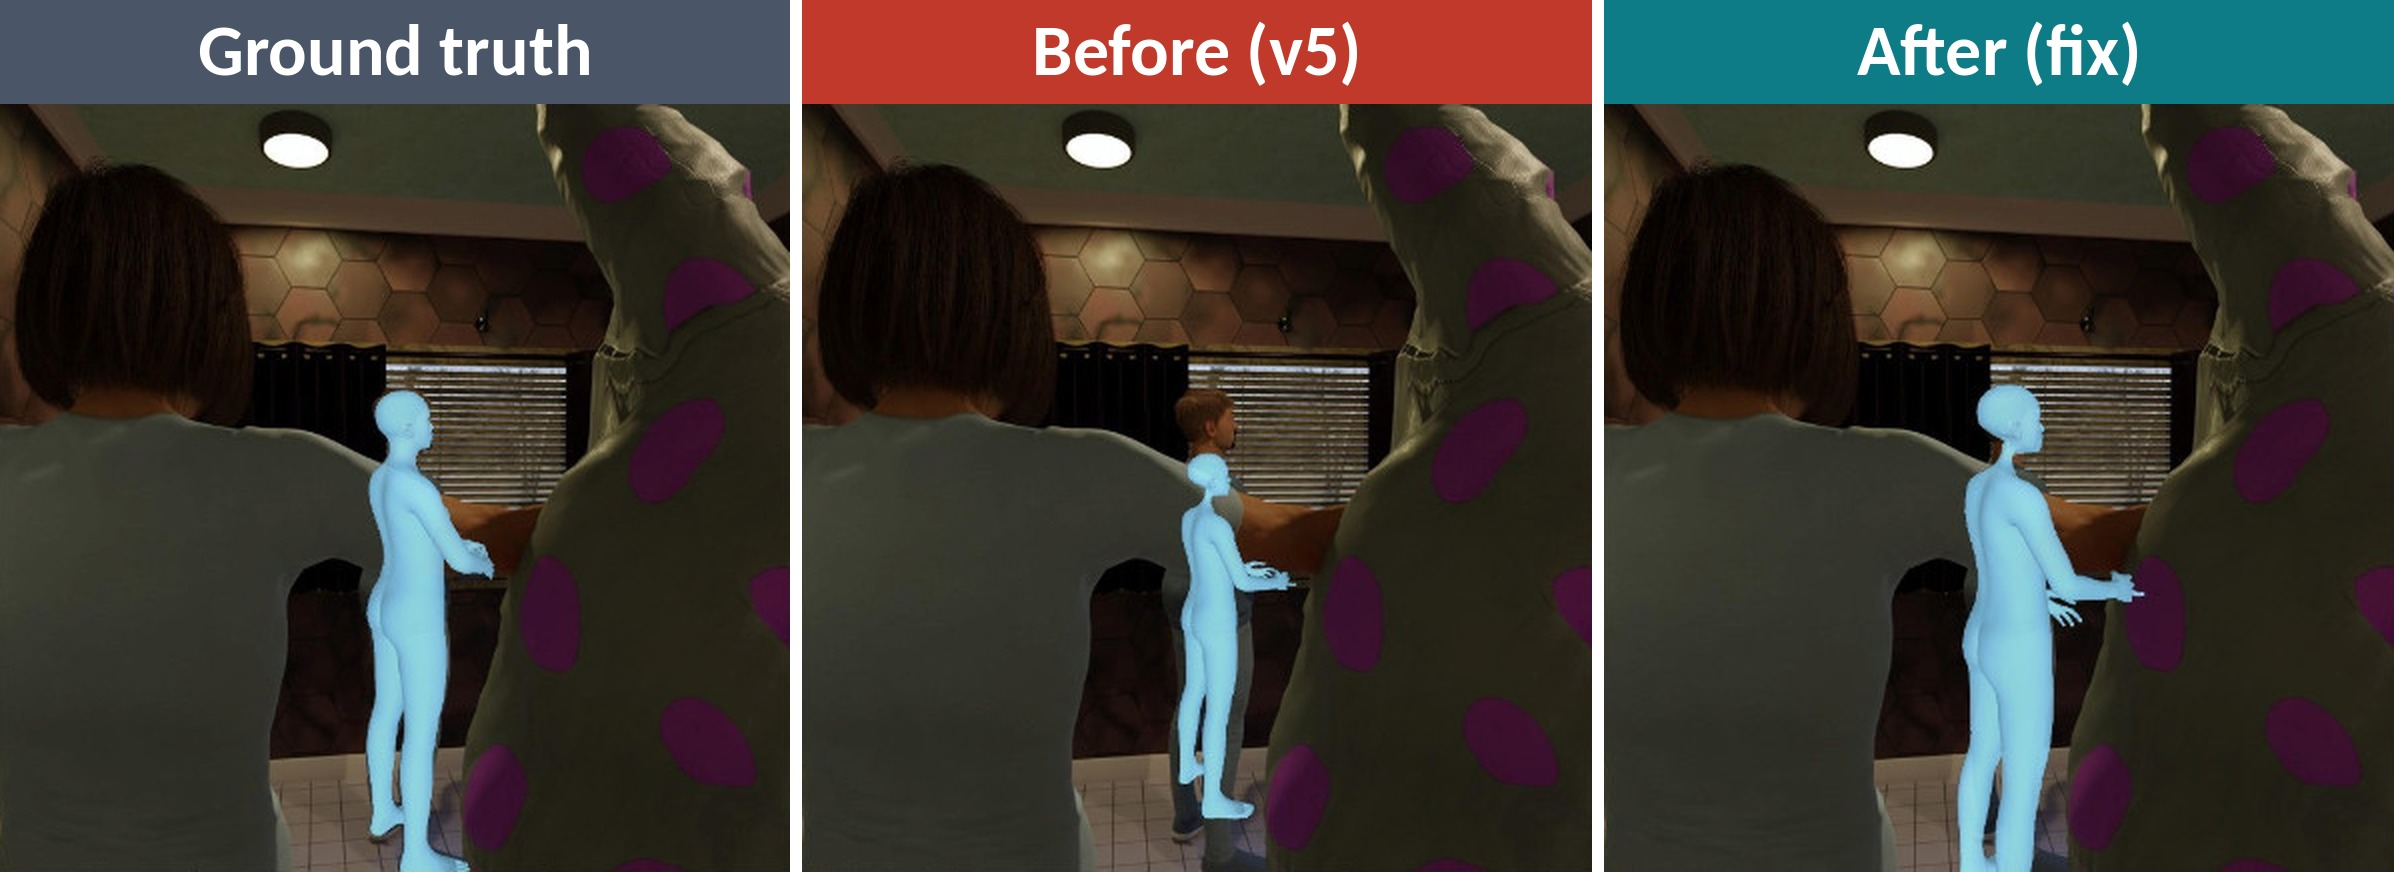
\includegraphics[width=0.9\linewidth]{depth_before_after_579860}
\caption[Holdout image 579860 at the predicted depth: ground truth, Base, depth pilot]{Holdout image 579860
rendered at each model's own predicted depth: ground truth, Base, and the depth pilot (head-joint targets, depth
weight $\times$5, 10 epochs, AnnyOne only). Before the fix the ground-truth head shows above a shrunken body placed
too far away. Synthetic image; one case, not a typical one. Companion of Figure~\ref{fig:depth-579862}.}
\label{fig:depth-579860}
\end{figure}

% F23: exp6 compare panels on the holdout (Base without and with the bone correction, no training; job in Appendix A).
\begin{figure}[tbp]
\centering
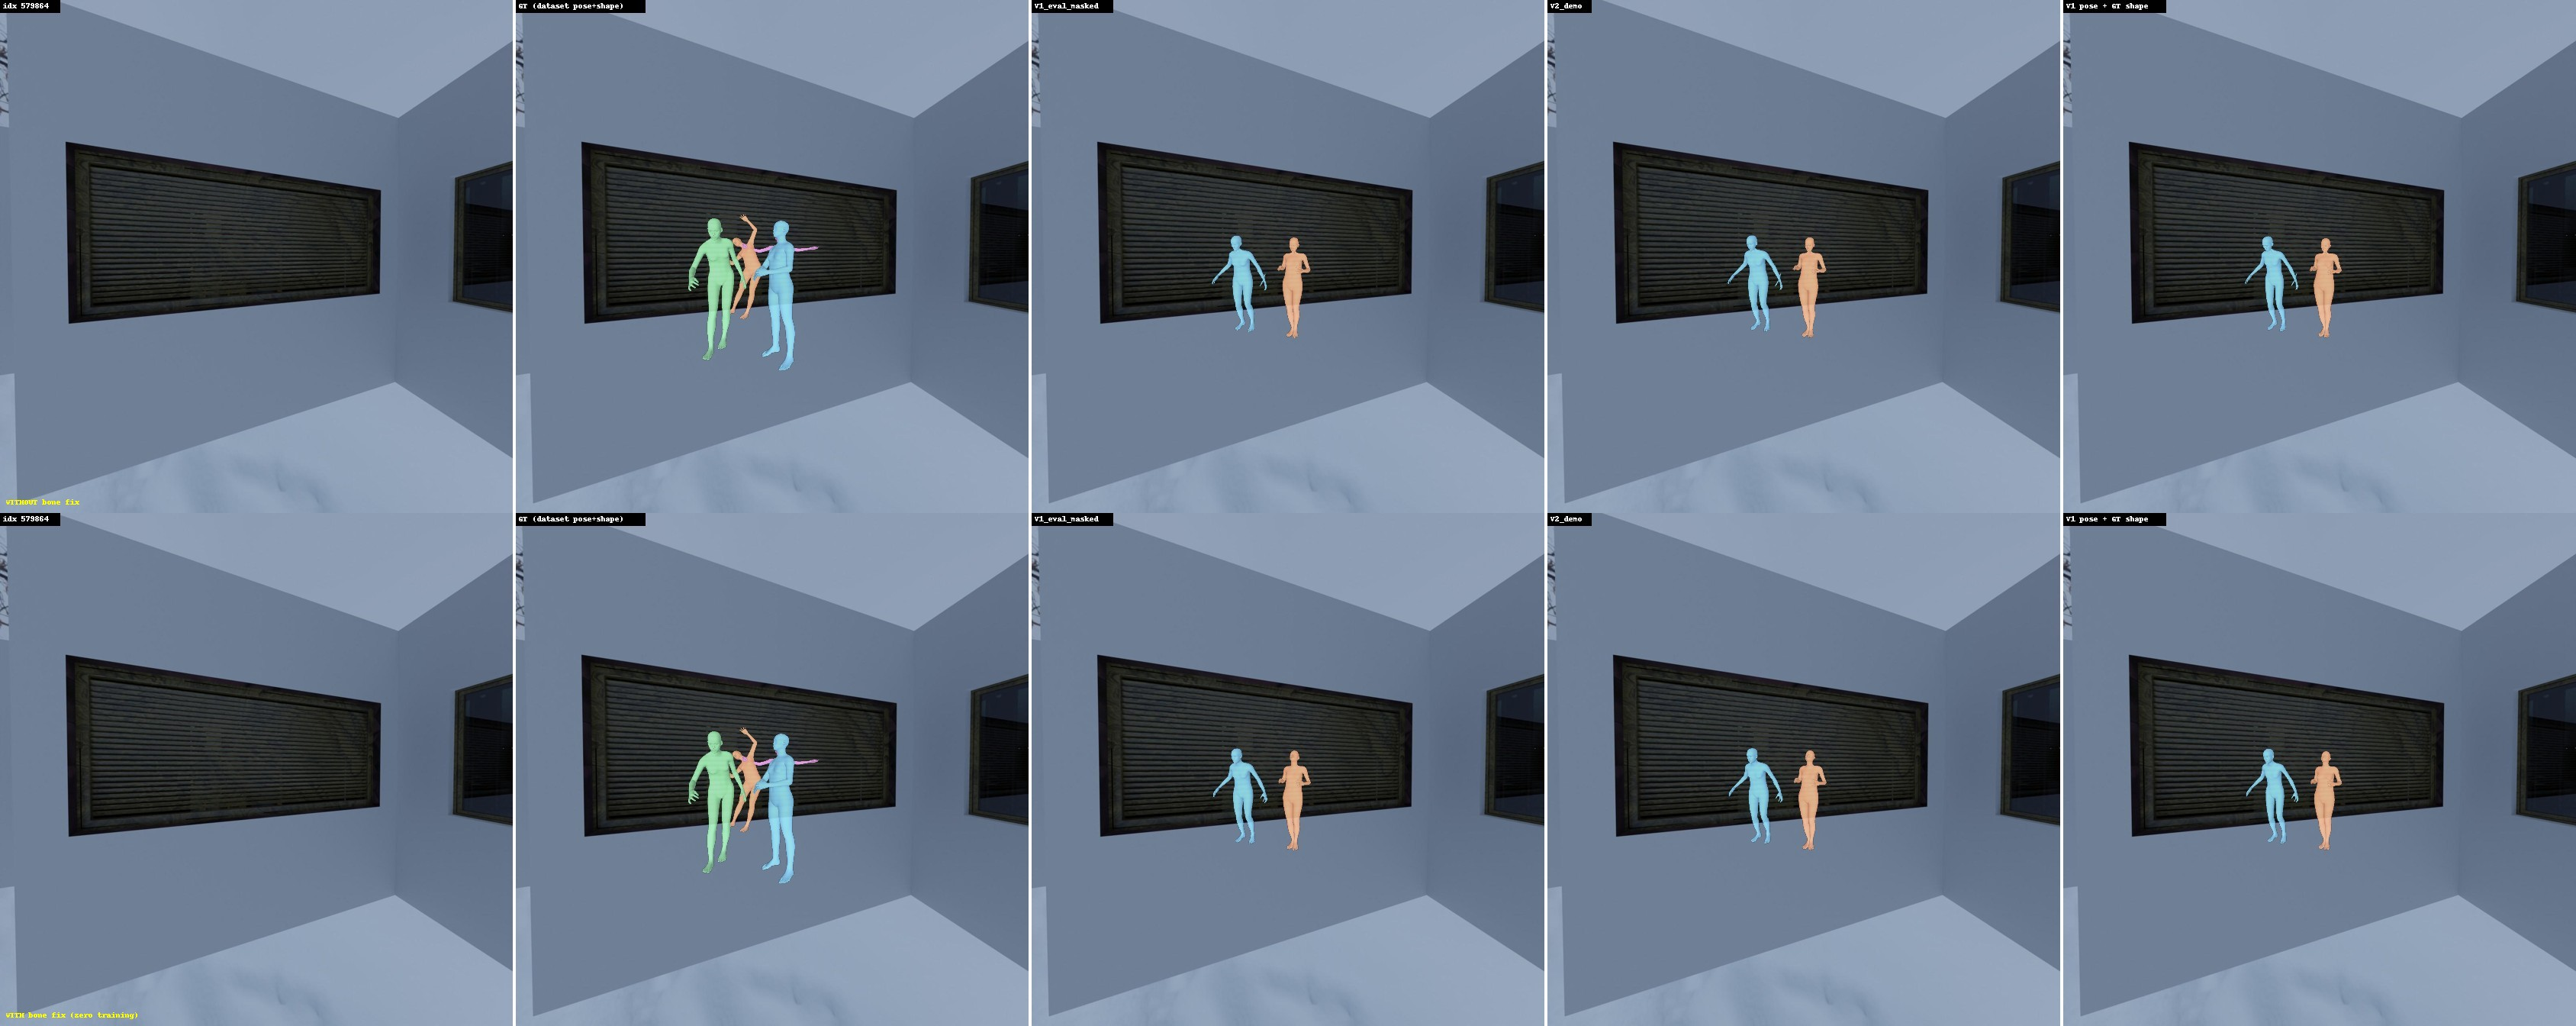
\includegraphics[width=0.49\linewidth]{exp6_compare_579864}\hfill
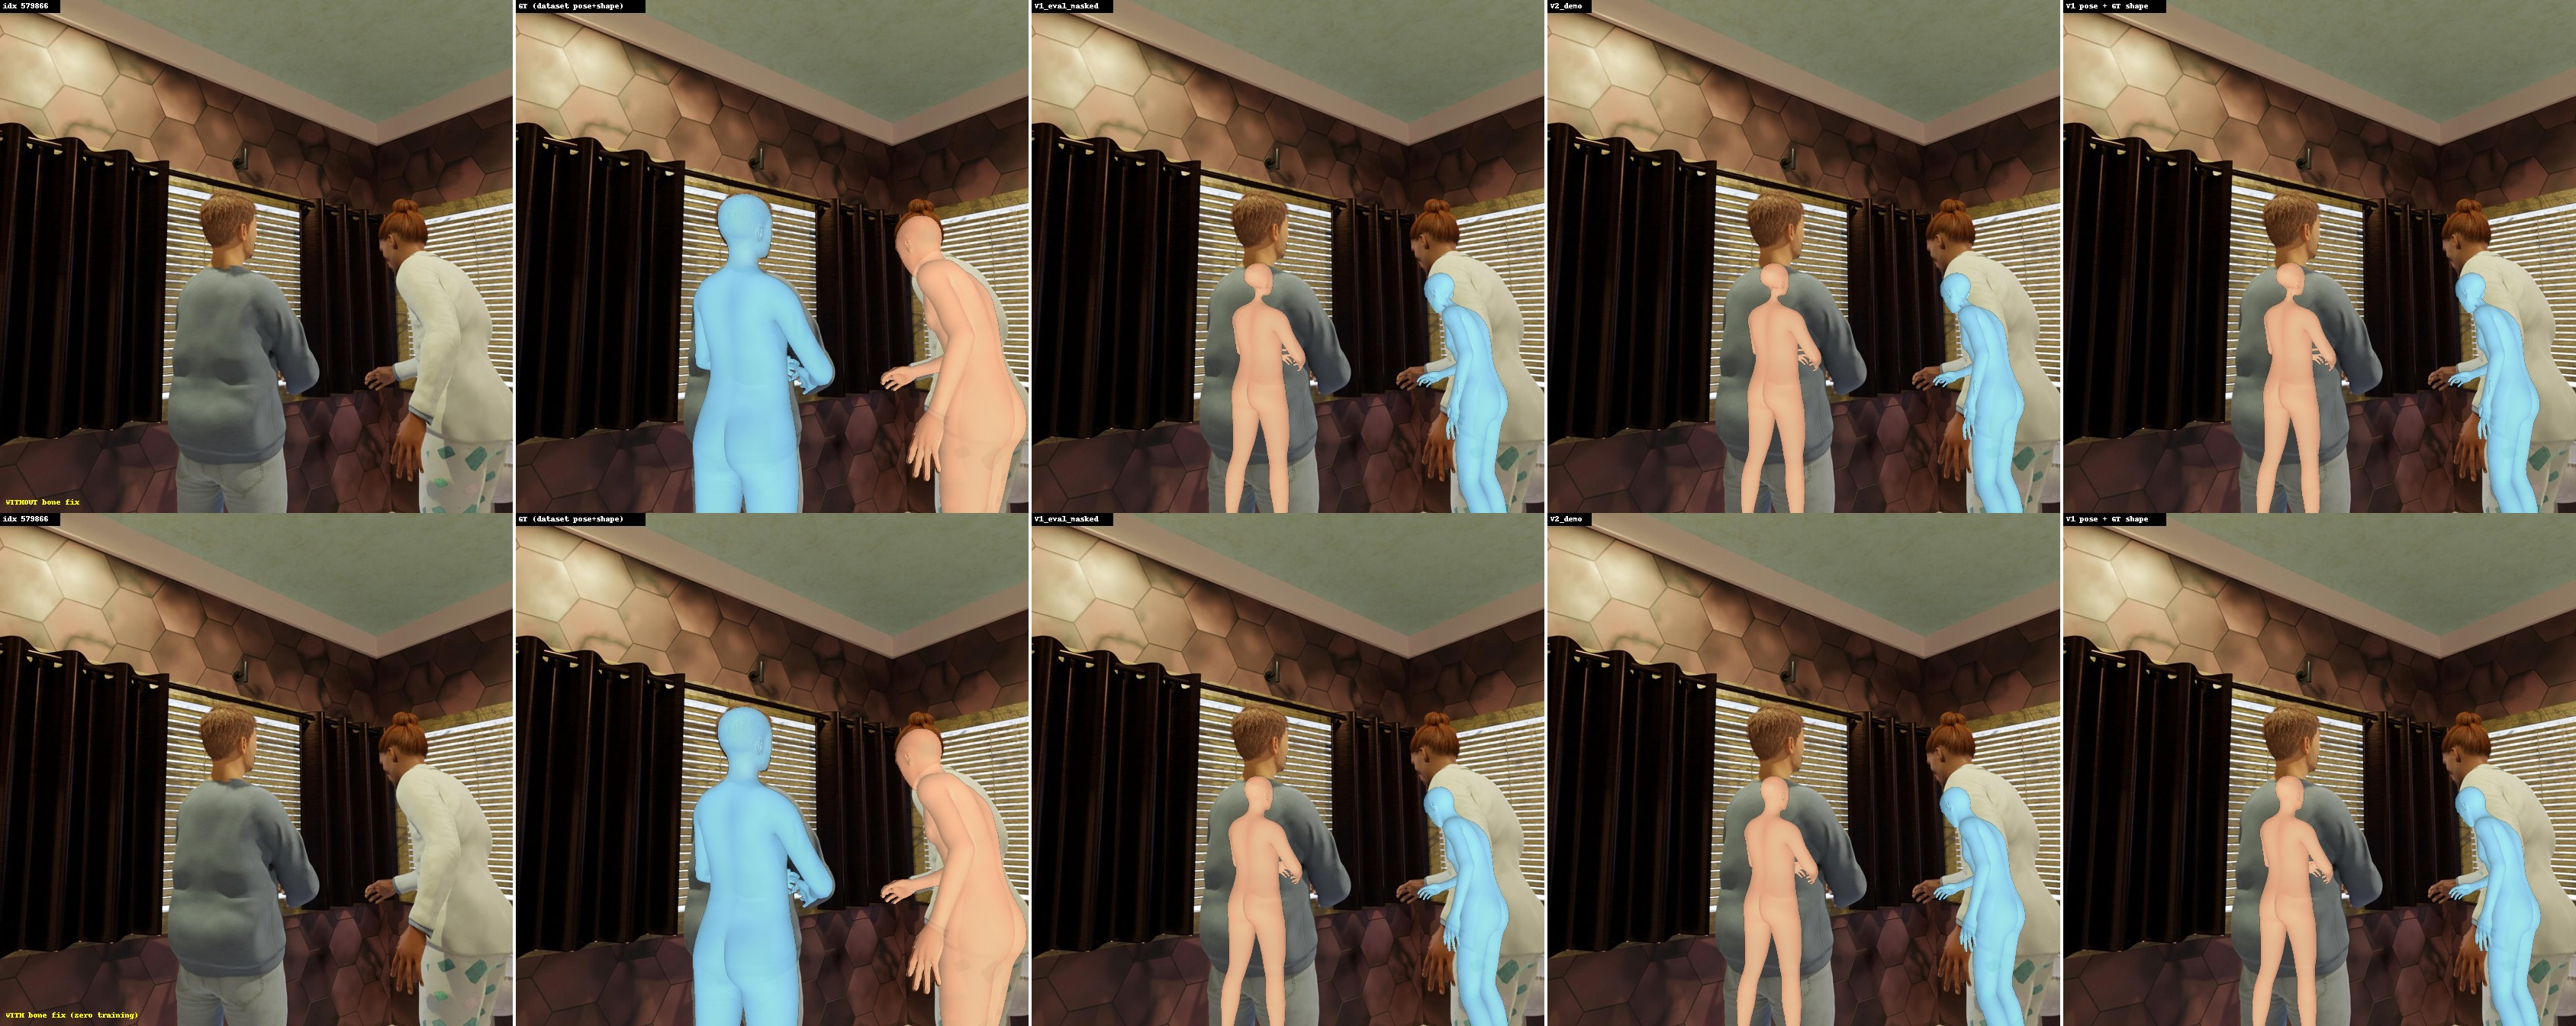
\includegraphics[width=0.49\linewidth]{exp6_compare_579866}
\caption[Two more holdout pairs: Base without and with the bone correction]{Holdout images 579864 (left) and 579866
(right): Base as trained next to the same checkpoint with the bone correction applied at the output, no training
(Section~\ref{sec:diag-neck}). Synthetic images, bodies at the model's own predicted depth, so the depth bug still
draws them too small; necks judged by eye. Companions of Figure~\ref{fig:diag-neck-base}.}
\label{fig:exp6-compare}
\end{figure}

% F9 office pair (plan section 3). Source docs/figures/neck_before_after_3dpw_bar_office.jpg.
\begin{figure}[tbp]
\centering
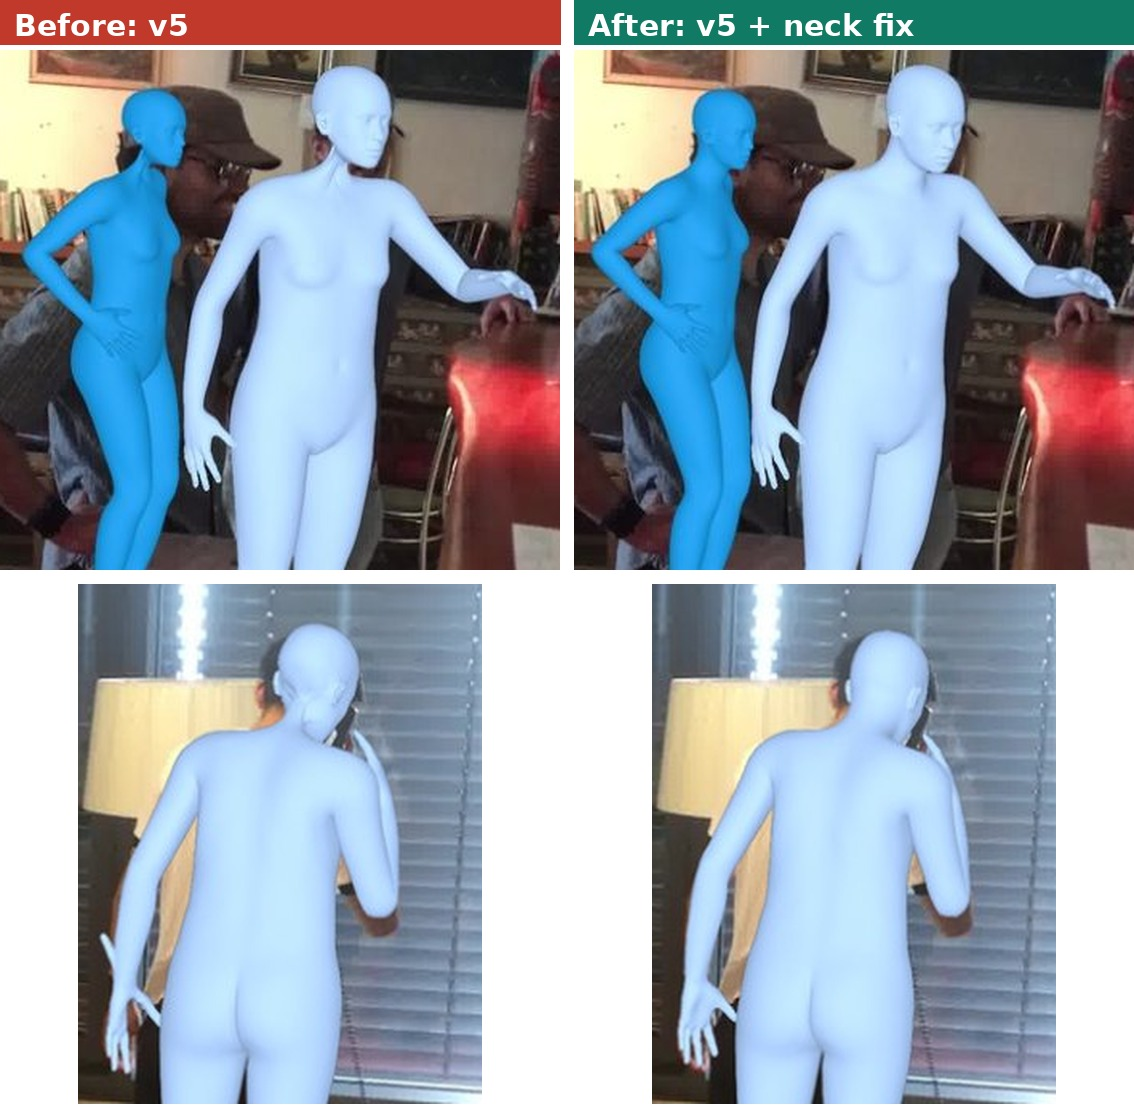
\includegraphics[width=0.9\linewidth]{neck_before_after_3dpw_bar_office}
\caption[Two 3DPW test frames: Base against the neck pilot]{Real 3DPW test frames \texttt{downtown\_bar\_00} 701
(top) and \texttt{office\_phoneCall\_00} 440 (bottom): Base next to the neck pilot (the bone correction and a 2-epoch
fine-tune); necks ringed. Bodies placed from the detector box, fingers at rest pose; judged by eye, no metric. The two
columns differ by the correction and by the fine-tune.}
\label{fig:neck-3dpw-office}
\end{figure}

% F10, the other four 3DPW test frames of the demo (photo | Base | photo | Final, labels baked into the image).
\begin{figure}[tbp]
\centering
\begin{subfigure}{0.495\linewidth}\centering
  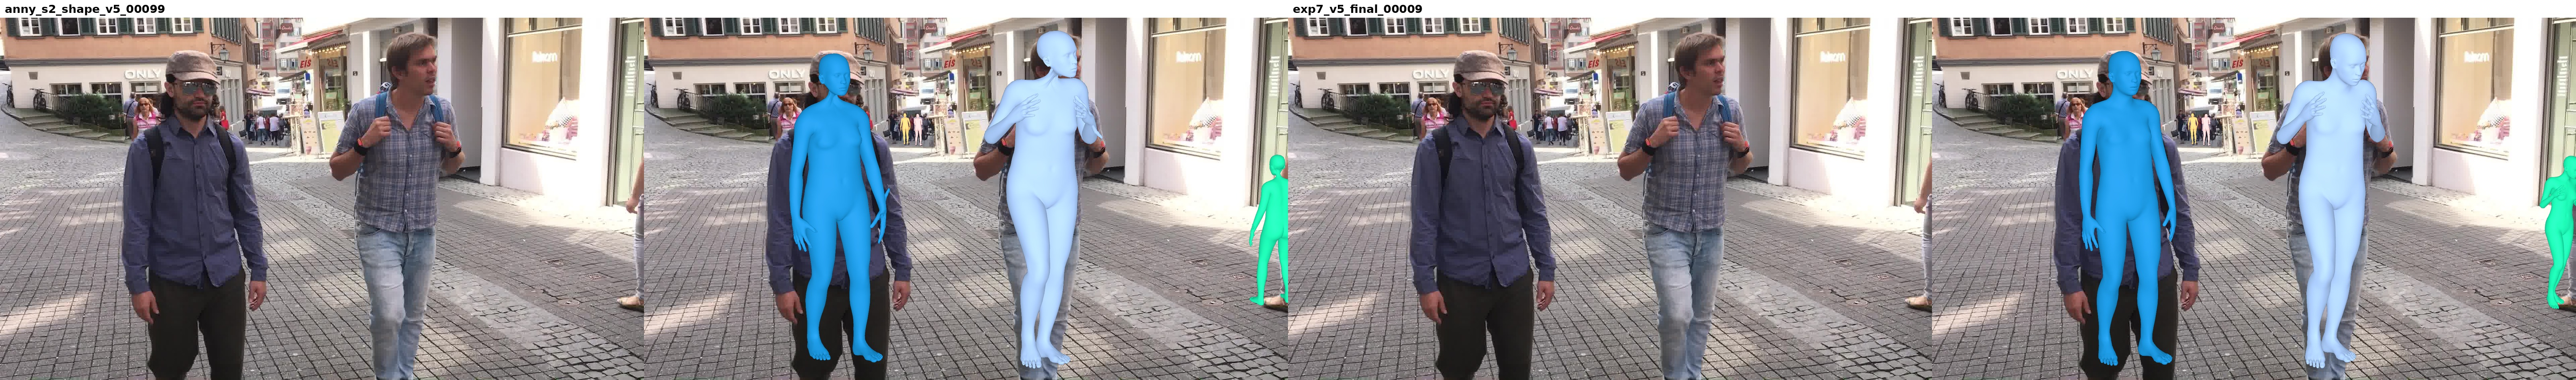
\includegraphics[width=\linewidth]{F10_3dpw_walking_v5_vs_final}\caption{\texttt{downtown\_walking}}\end{subfigure}\hfill
\begin{subfigure}{0.495\linewidth}\centering
  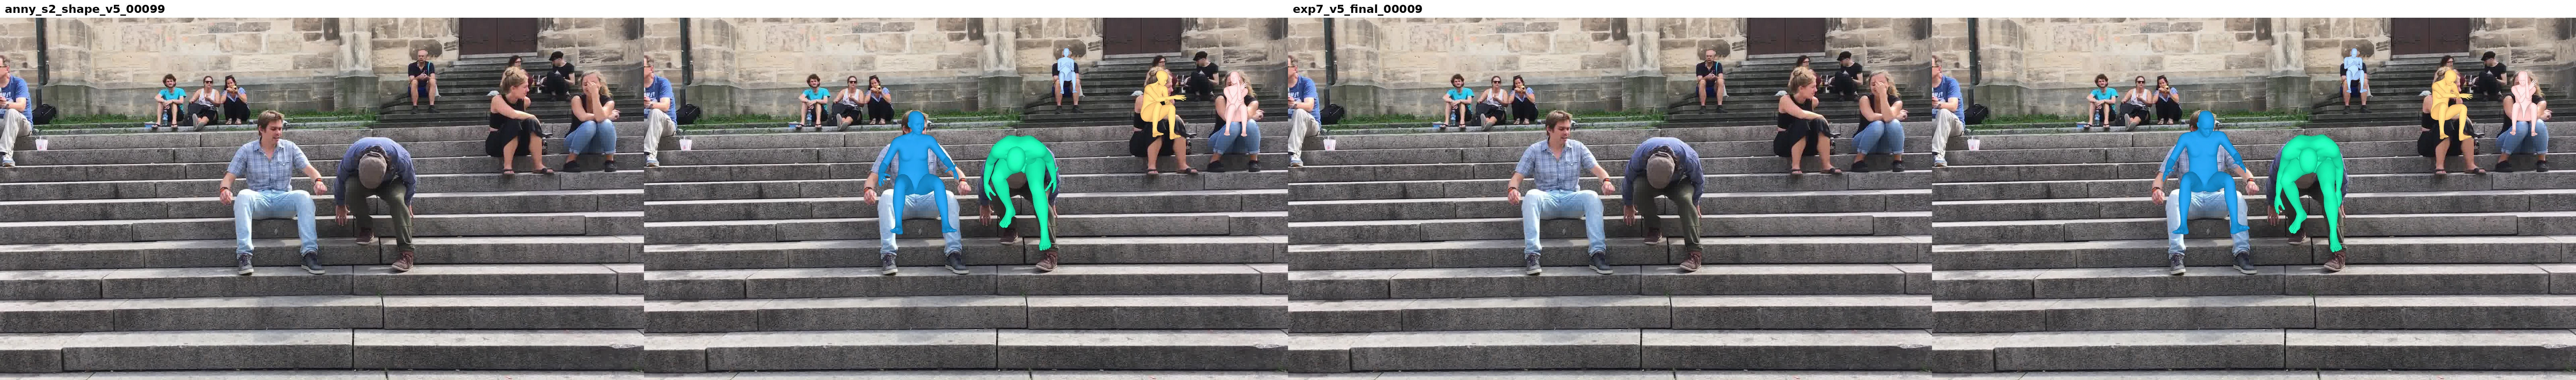
\includegraphics[width=\linewidth]{F10_3dpw_stairs_v5_vs_final}\caption{stairs}\end{subfigure}\\[4pt]
\begin{subfigure}{0.495\linewidth}\centering
  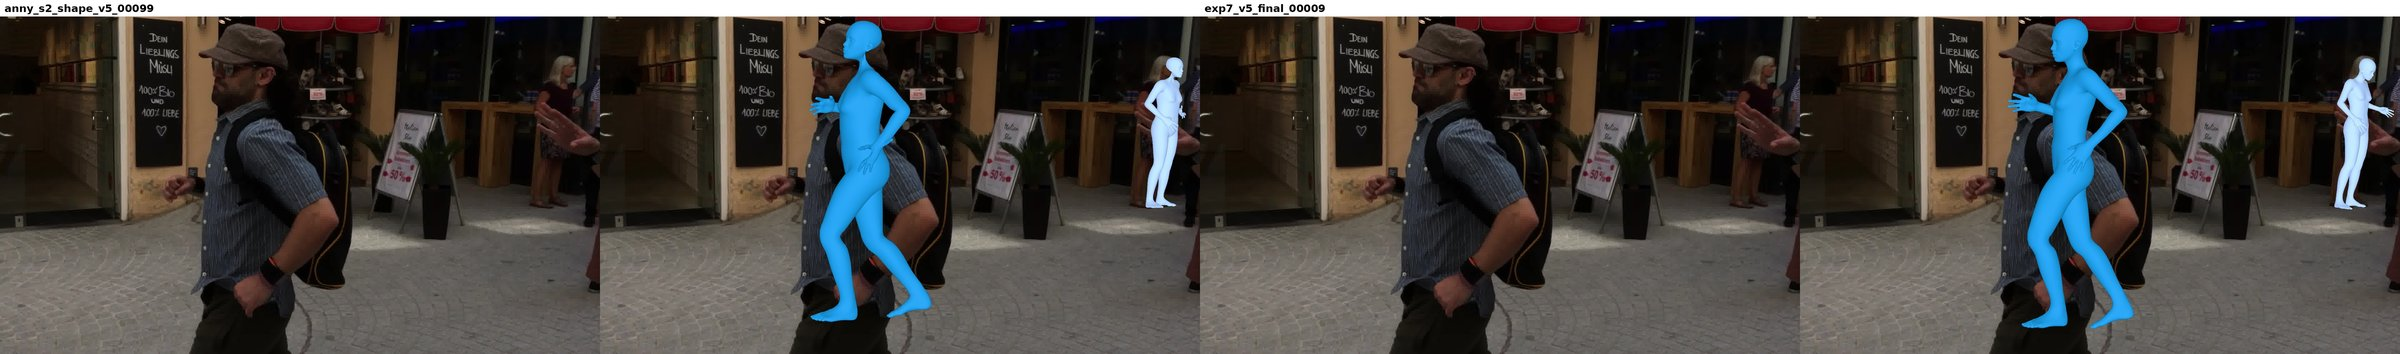
\includegraphics[width=\linewidth]{F10_3dpw_runforbus_v5_vs_final}\caption{\texttt{downtown\_runForBus}}\end{subfigure}\hfill
\begin{subfigure}{0.495\linewidth}\centering
  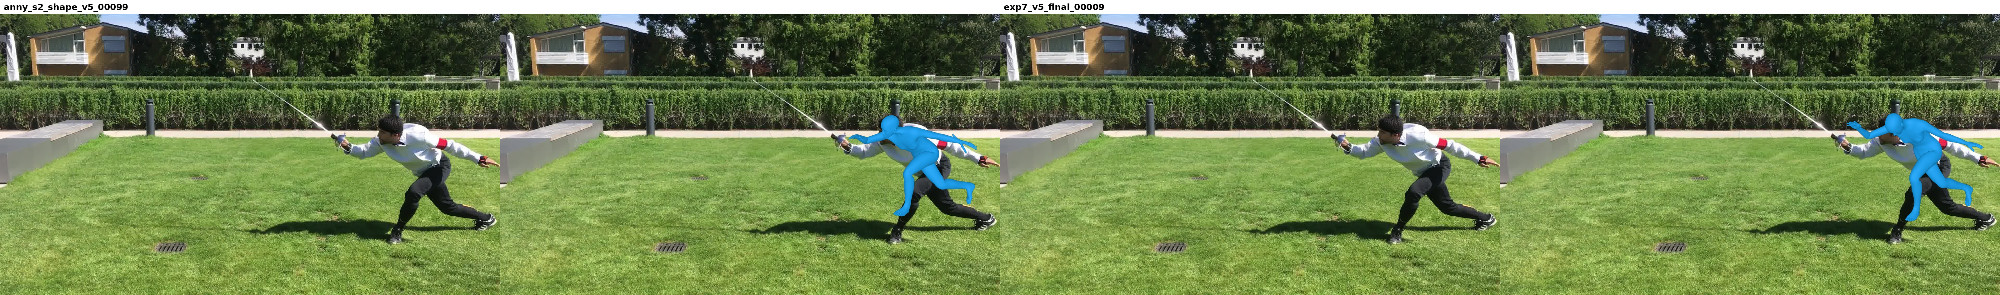
\includegraphics[width=\linewidth]{F10_3dpw_fencing_v5_vs_final}\caption{fencing}\end{subfigure}
\caption[Four more 3DPW test frames, Base against Final]{The other four 3DPW test frames of the demo, each shown as
photo and Base (left half), then photo and Final (right half; the labels in the image name the two checkpoints).
Bodies placed from the detector box, fingers at rest pose; judged by eye, no metric. The first four frames are in
Figure~\ref{fig:3dpw-overlays}.}
\label{fig:3dpw-overlays-more}
\end{figure}

% F10 photo montages (photo | Base | photo | Final, labels baked in).
\begin{figure}[tbp]
\centering
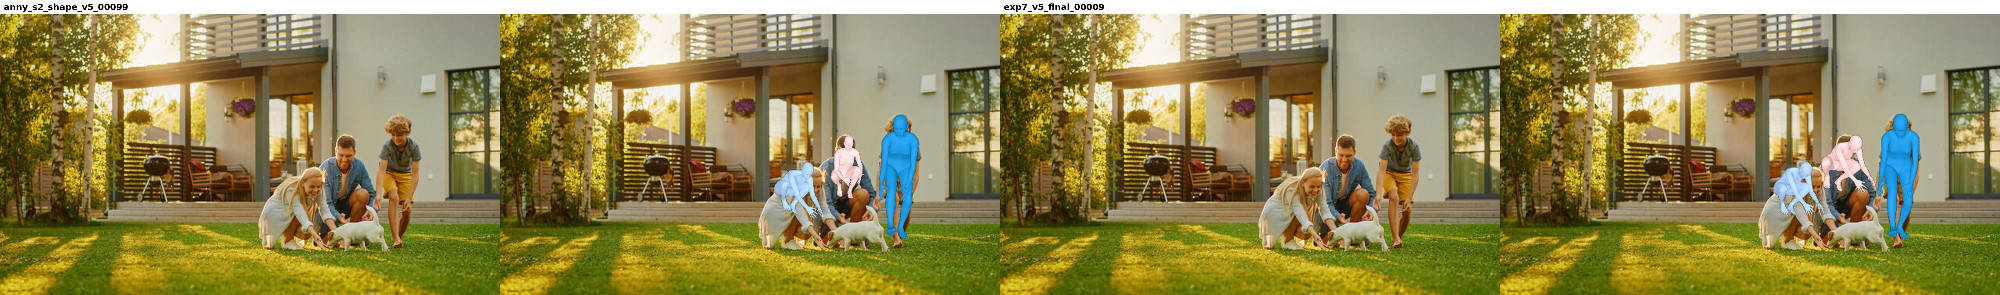
\includegraphics[width=\linewidth]{F10_photo_garden_v5_vs_final}\\[2pt]
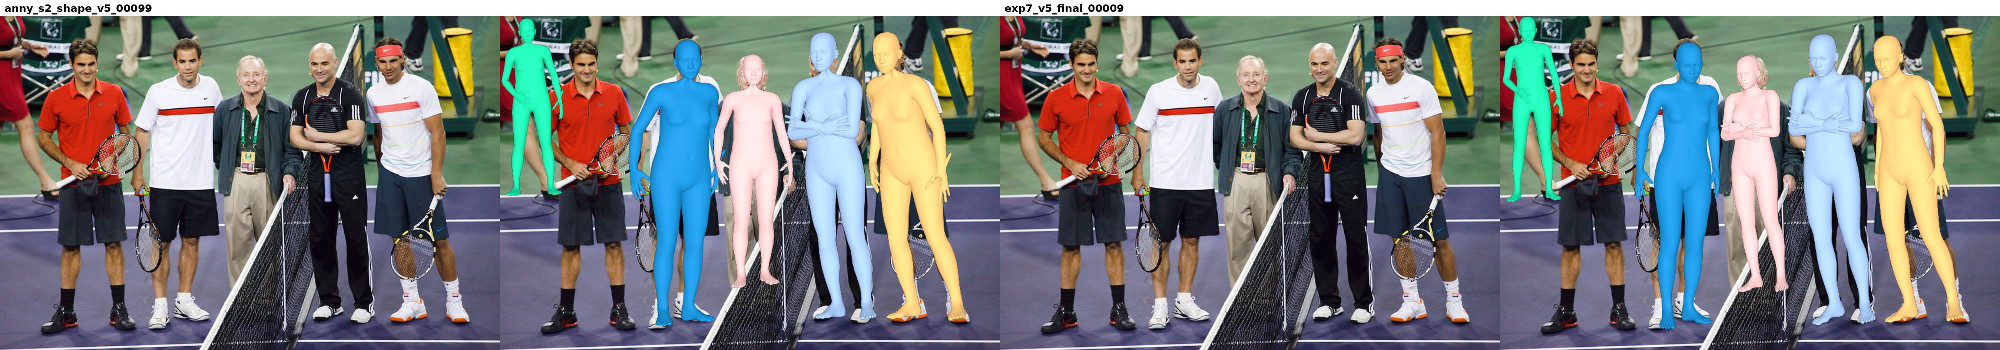
\includegraphics[width=\linewidth]{F10_photo_tennis_v5_vs_final}\\[2pt]
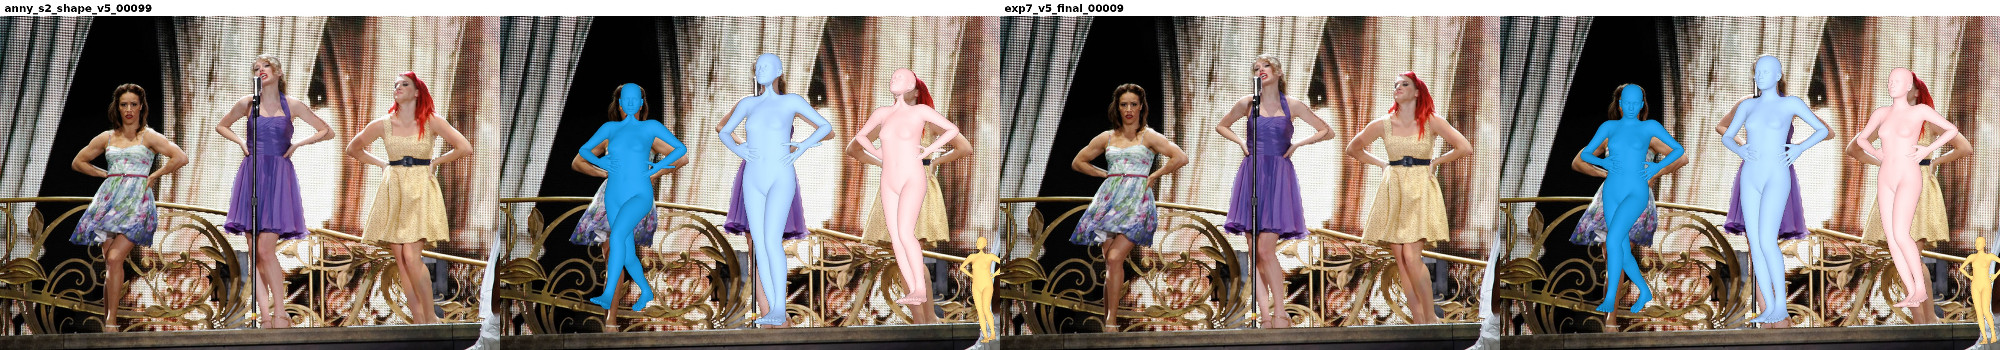
\includegraphics[width=\linewidth]{F10_photo_stage_v5_vs_final}\\[2pt]
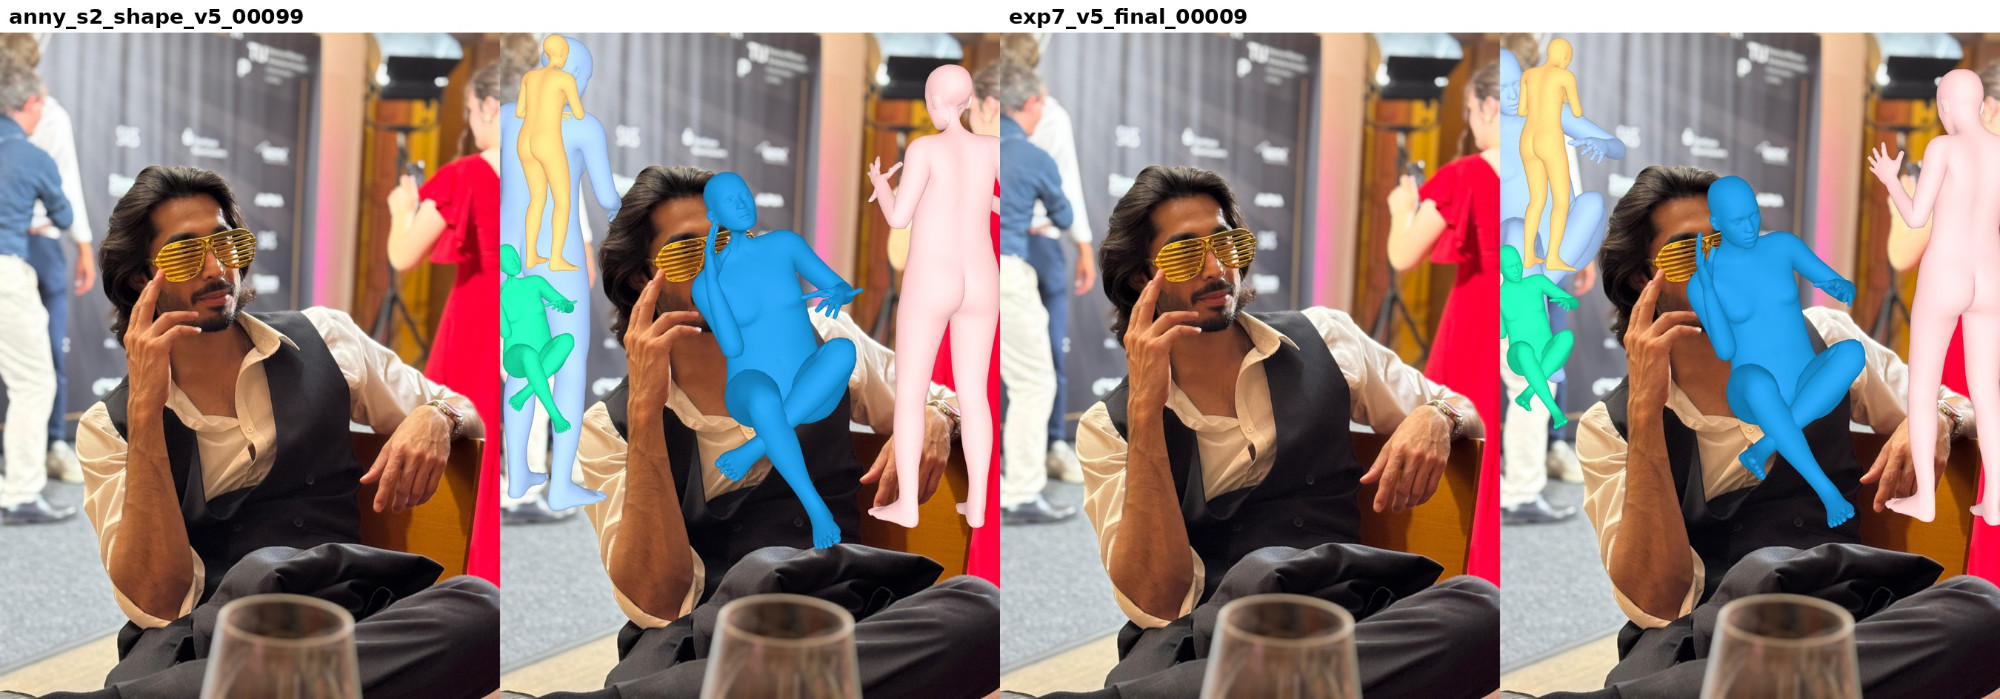
\includegraphics[width=\linewidth]{F10_photo_party_v5_vs_final}
\caption[Four real photos, Base against Final]{The four real photos of the demo (garden, tennis, stage, party), never
used in training, each shown as photo and Base, then photo and Final; bodies placed from the detector box, fingers at
rest pose; judged by eye, no metric. The tennis photo also appears in Figure~\ref{fig:real-photos}.}
\label{fig:photo-montages}
\end{figure}

% F11, all twelve montages (photo | Base | photo | Final, labels baked in; demo with --relax_hands 0). Chapter 6
% shows zoomed crops of party, guitar and bar only.
\begin{figure}[p]
\centering
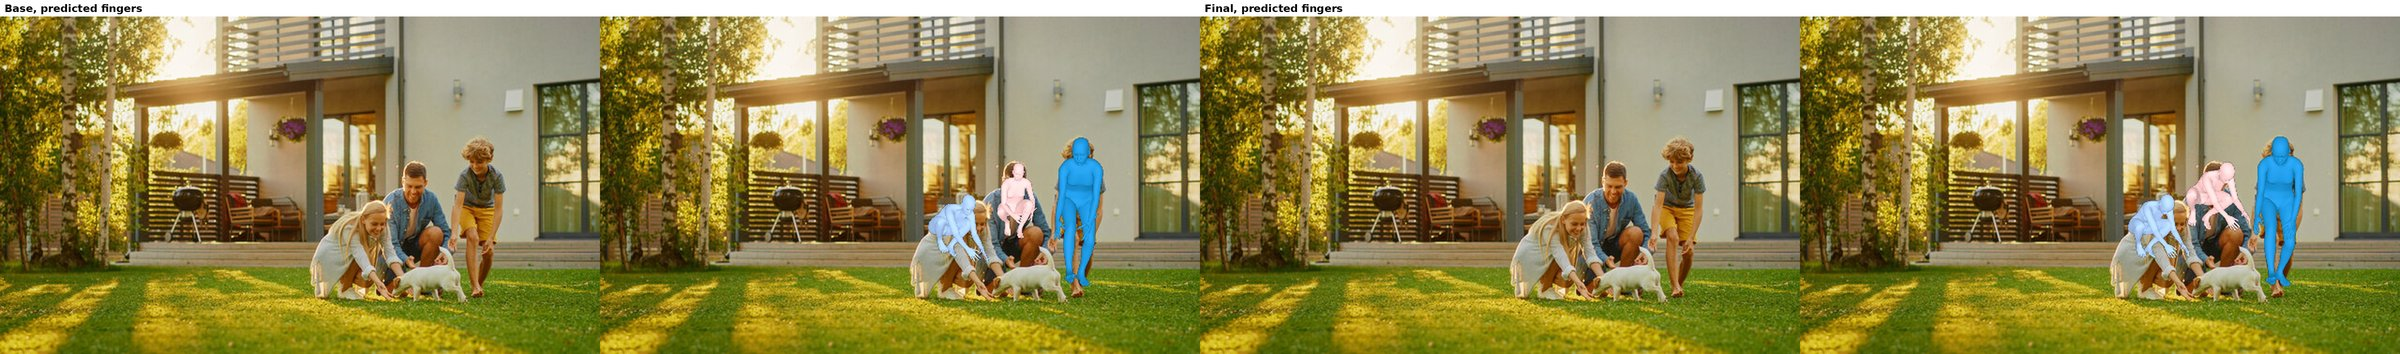
\includegraphics[width=0.82\linewidth]{F11_hands_photo_garden}\\[2pt]
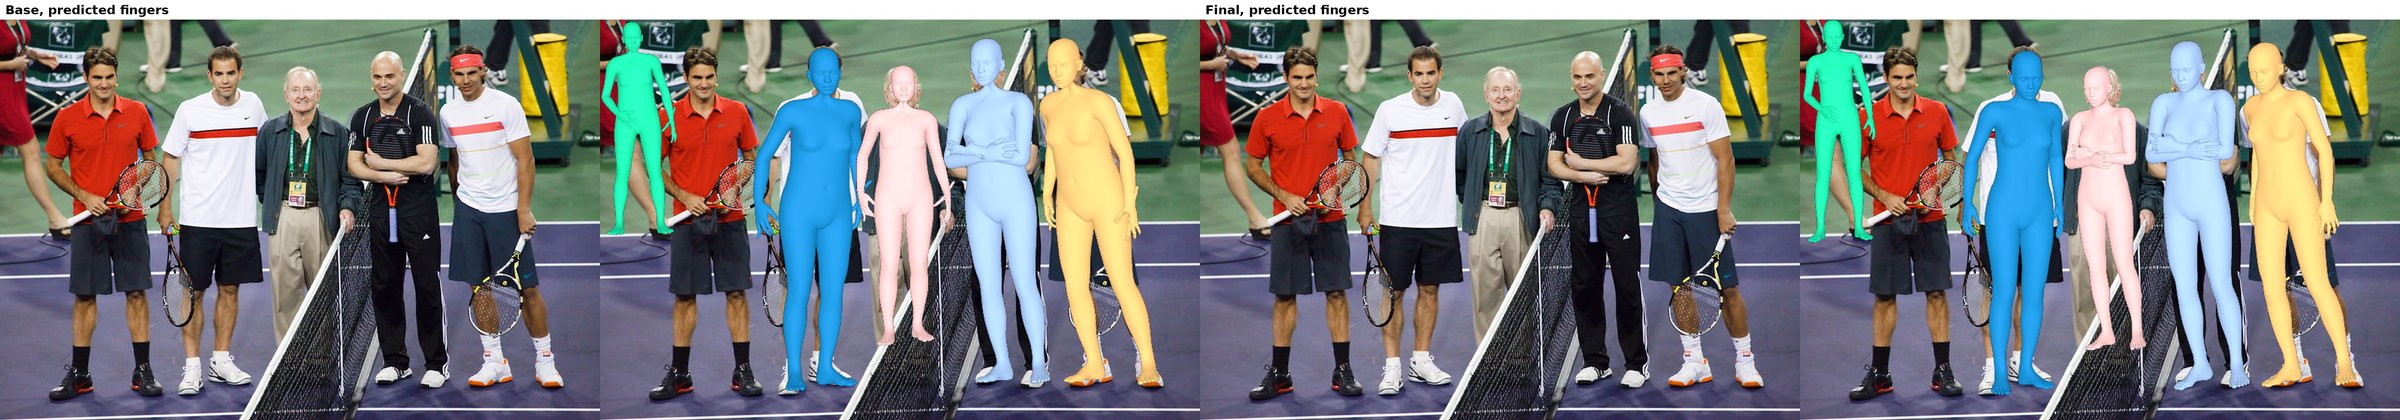
\includegraphics[width=0.82\linewidth]{F11_hands_photo_tennis}\\[2pt]
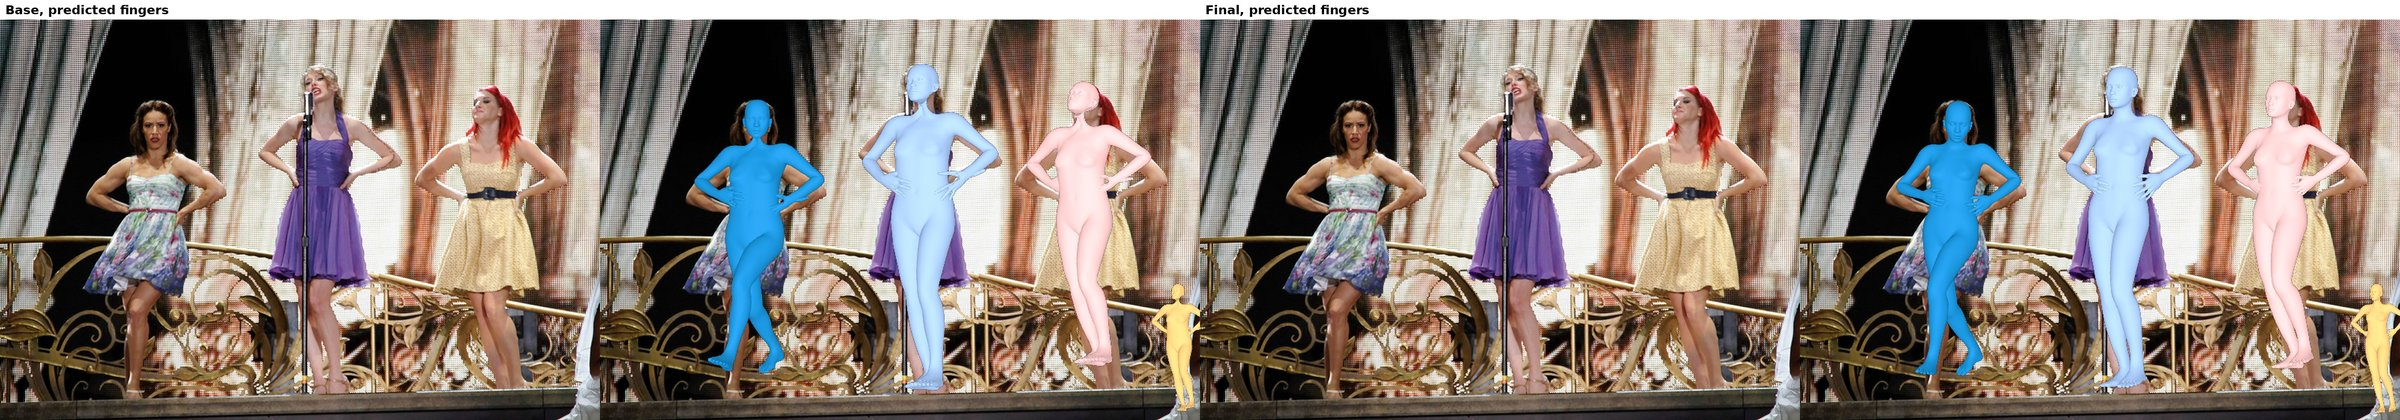
\includegraphics[width=0.82\linewidth]{F11_hands_photo_stage}\\[2pt]
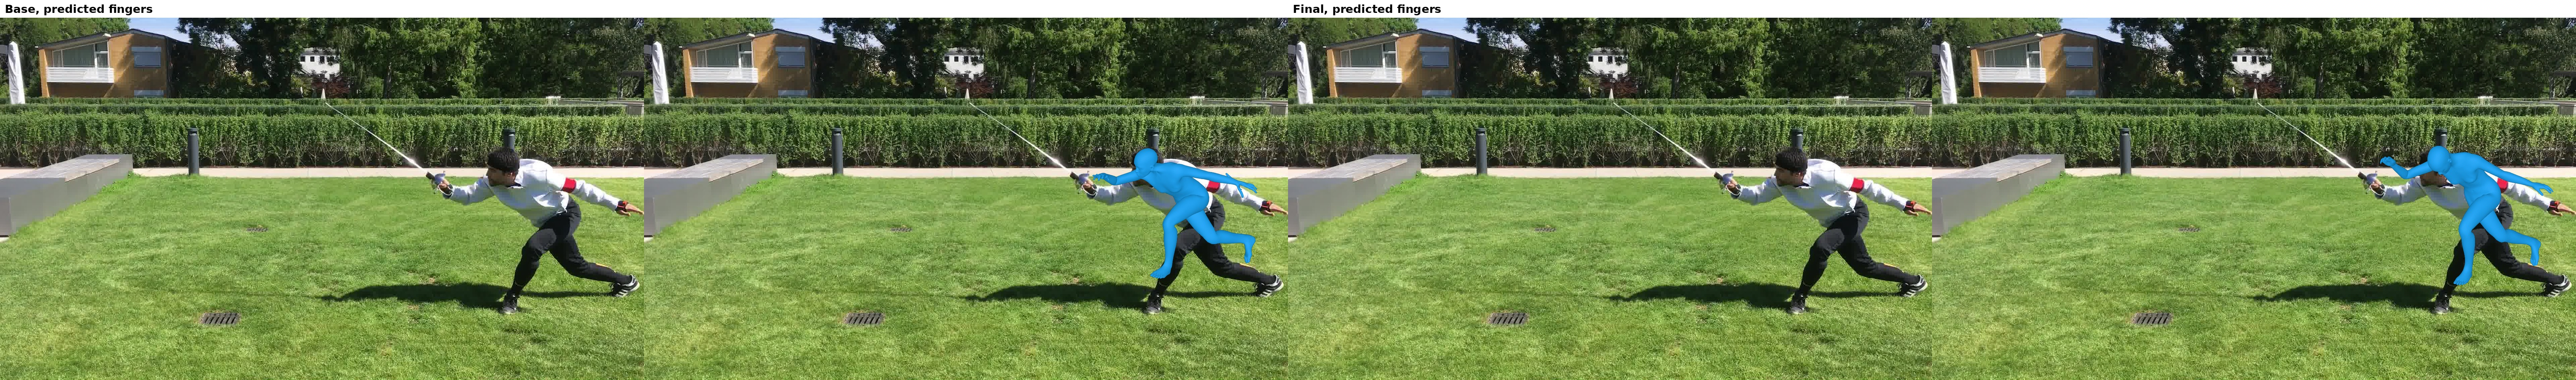
\includegraphics[width=0.82\linewidth]{F11_hands_3dpw_fencing}\\[2pt]
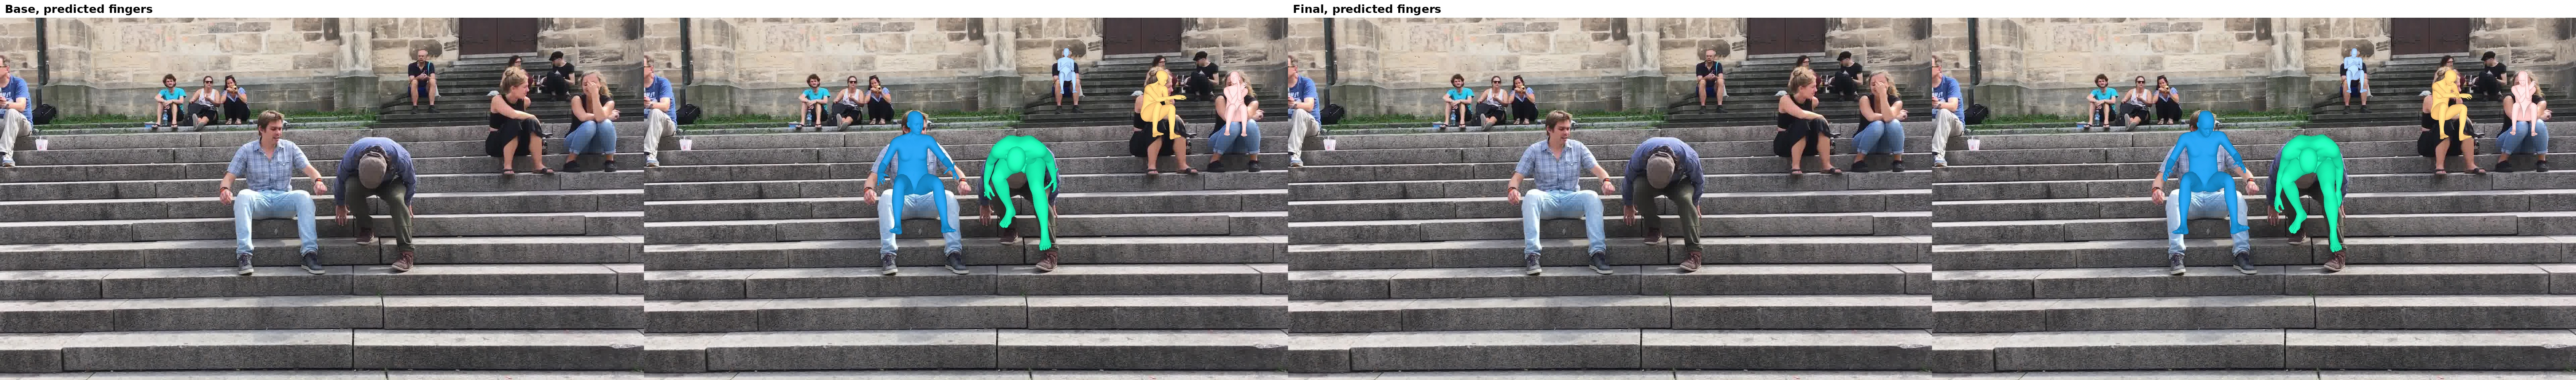
\includegraphics[width=0.82\linewidth]{F11_hands_3dpw_stairs}\\[2pt]
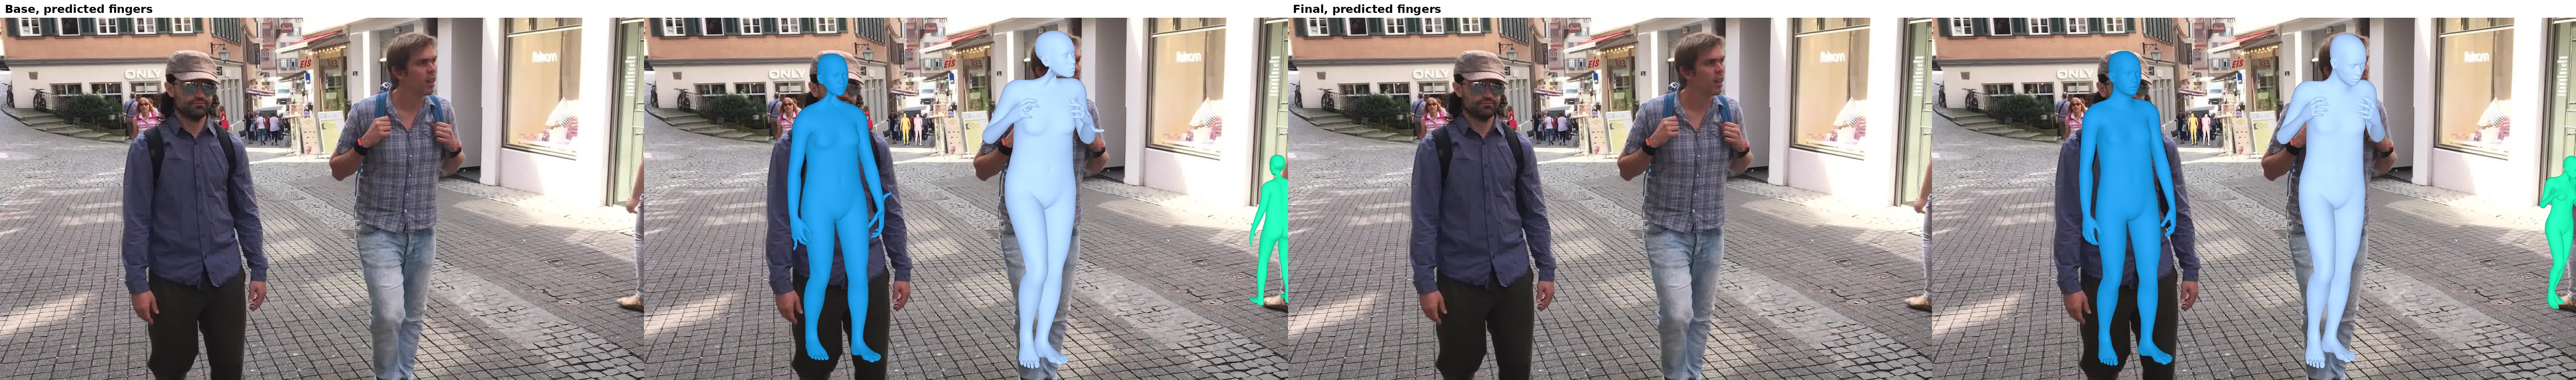
\includegraphics[width=0.82\linewidth]{F11_hands_3dpw_walking}\\[2pt]
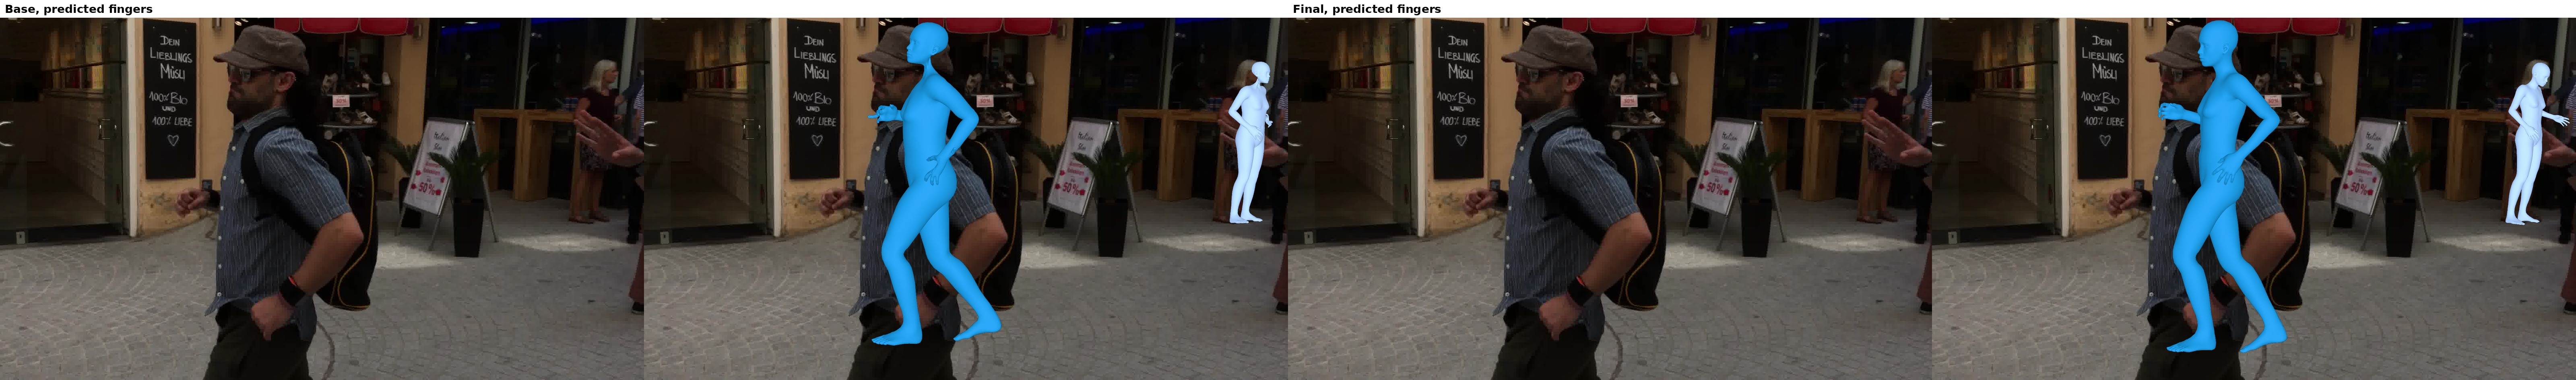
\includegraphics[width=0.82\linewidth]{F11_hands_3dpw_runforbus}\\[4pt]
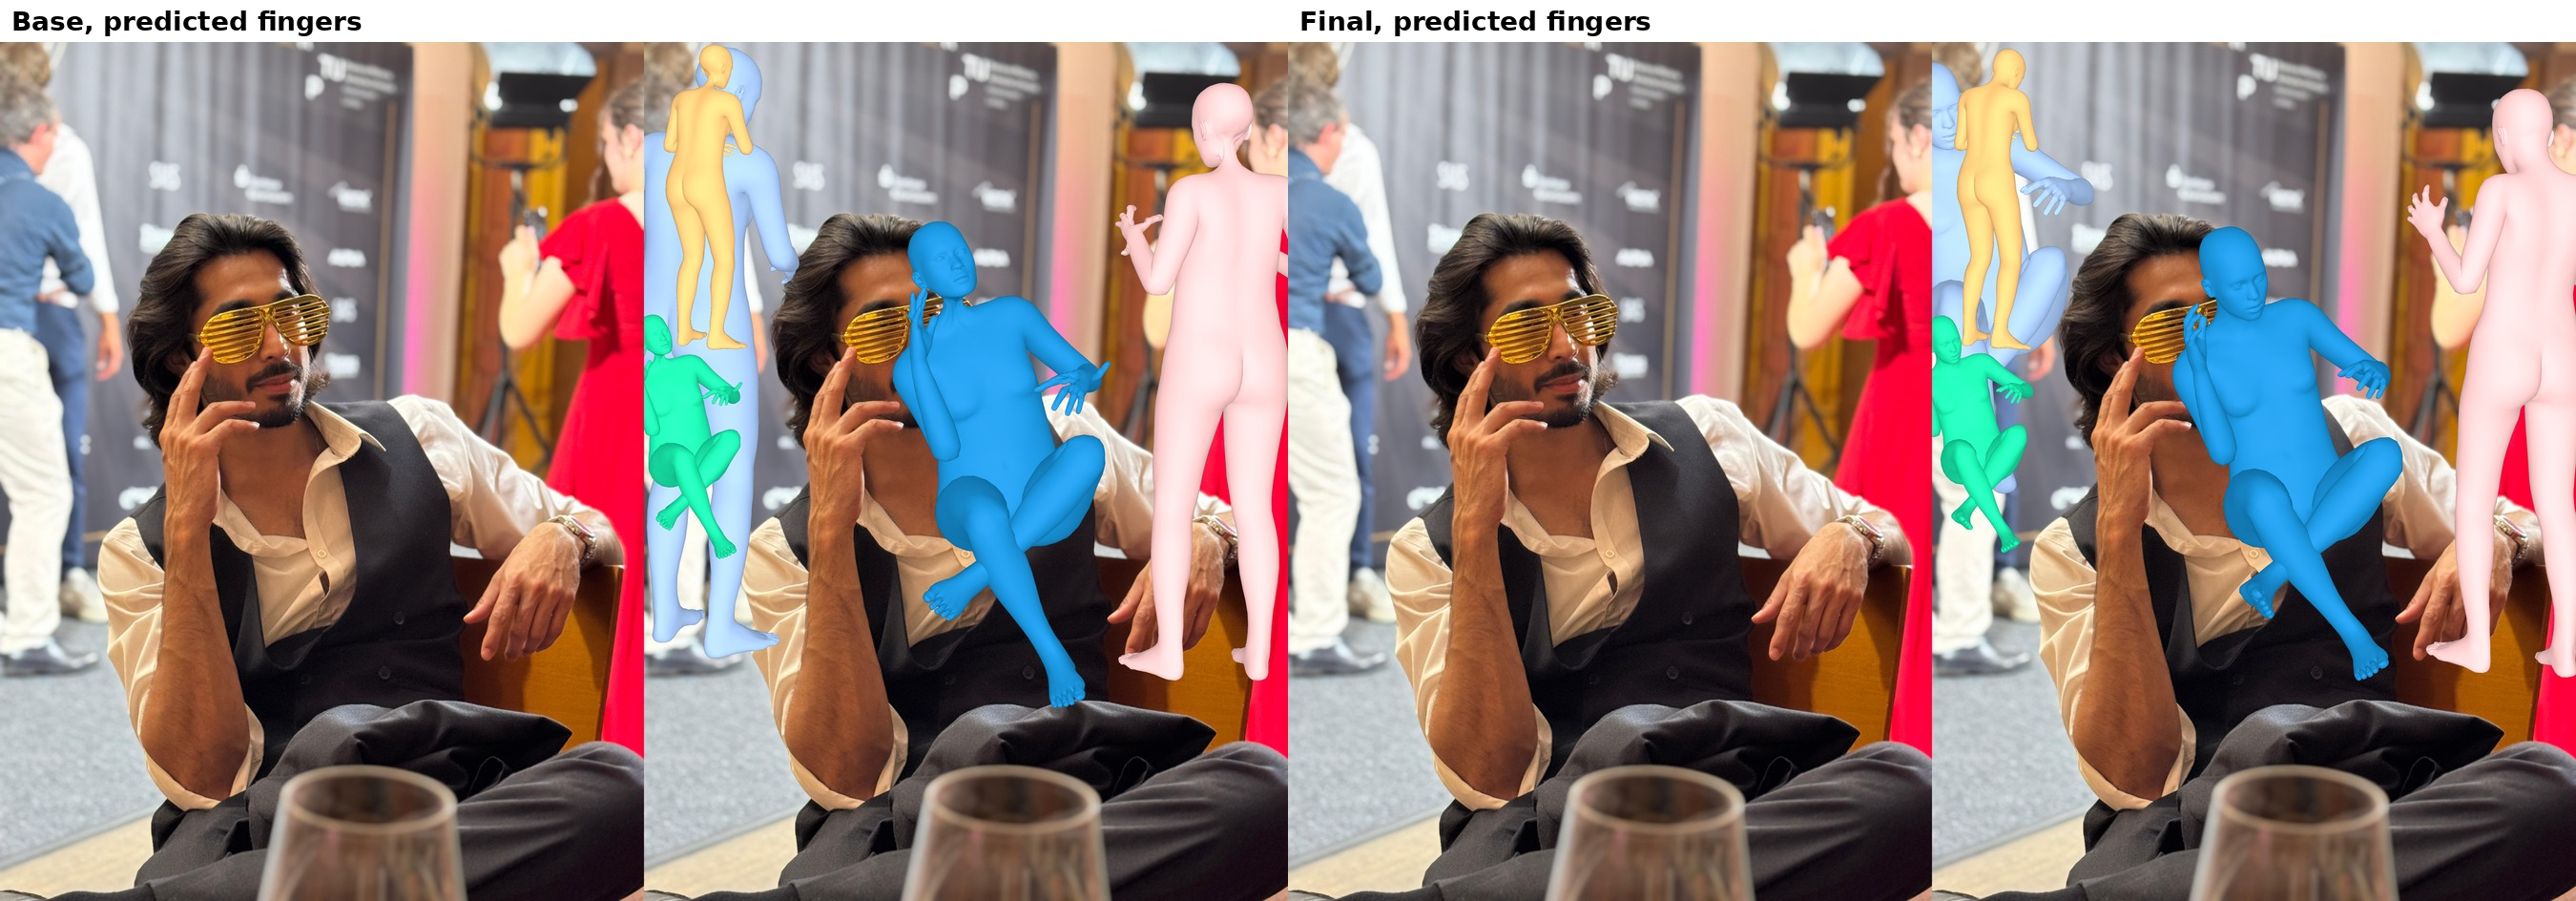
\includegraphics[width=0.385\linewidth]{F11_hands_photo_party}\hspace{2pt}%
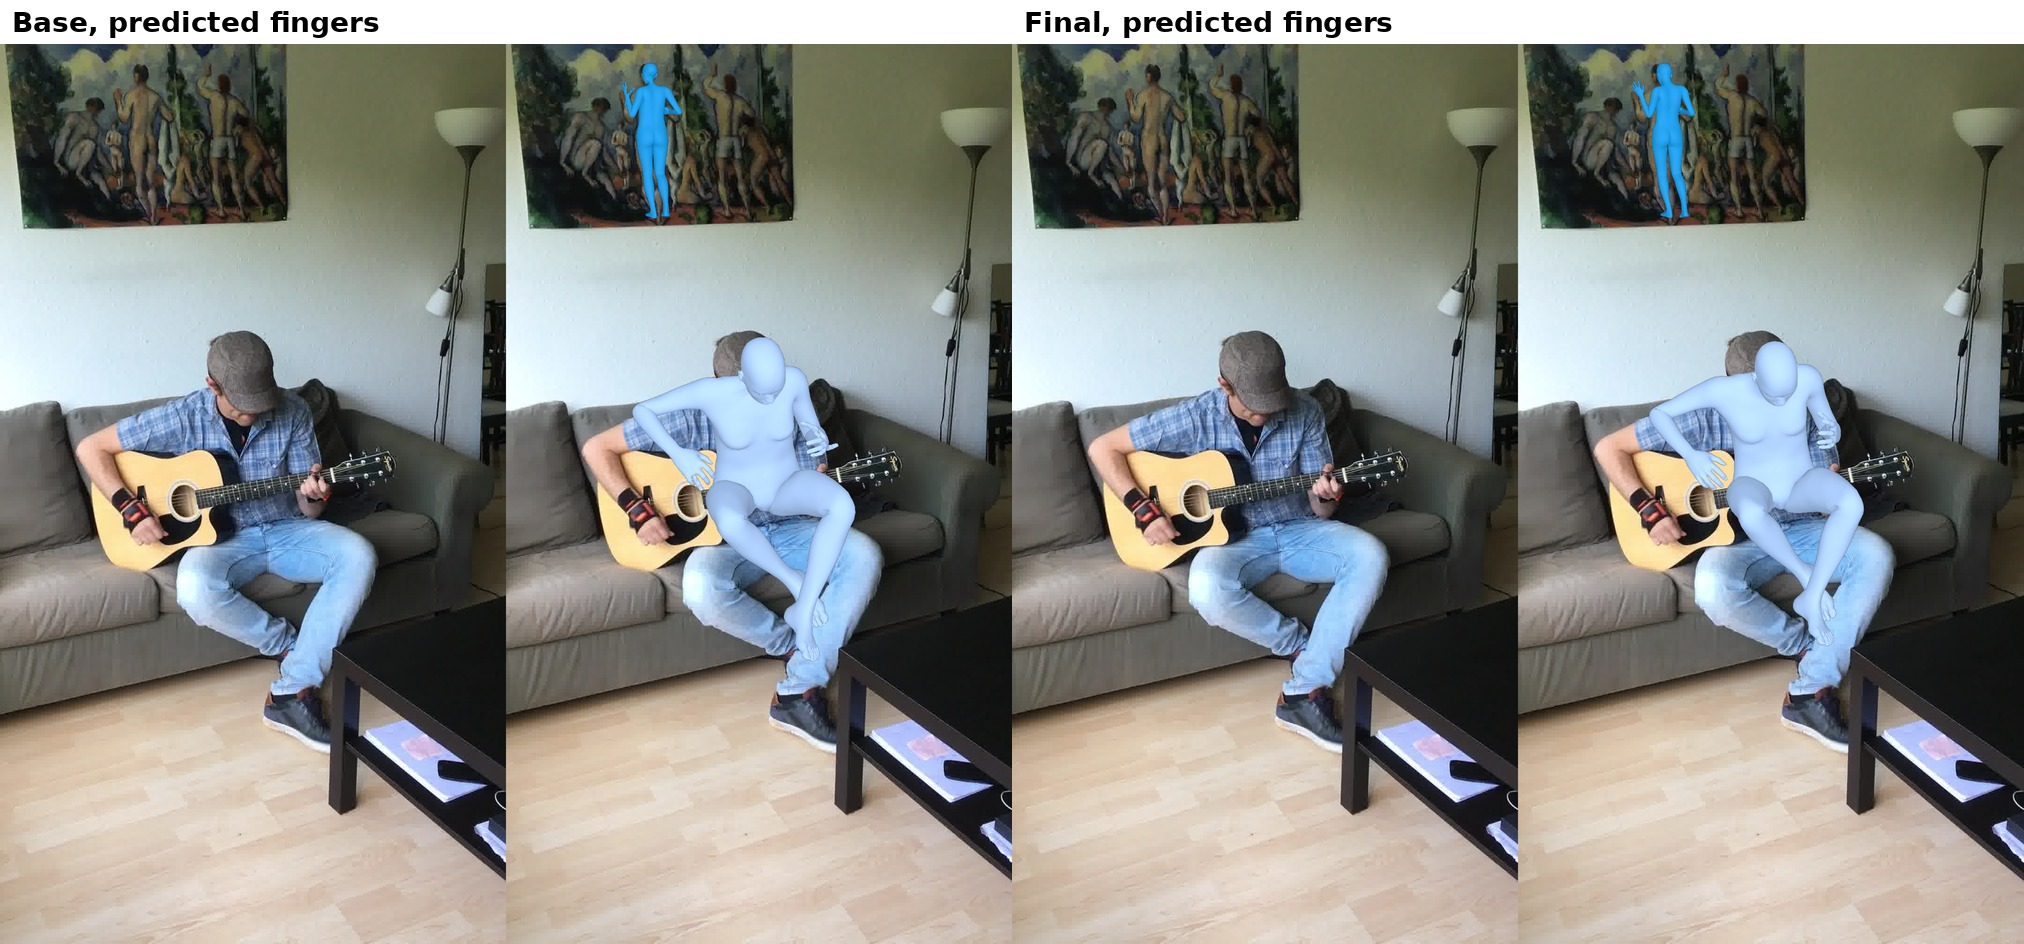
\includegraphics[width=0.288\linewidth]{F11_hands_3dpw_guitar}\hspace{2pt}%
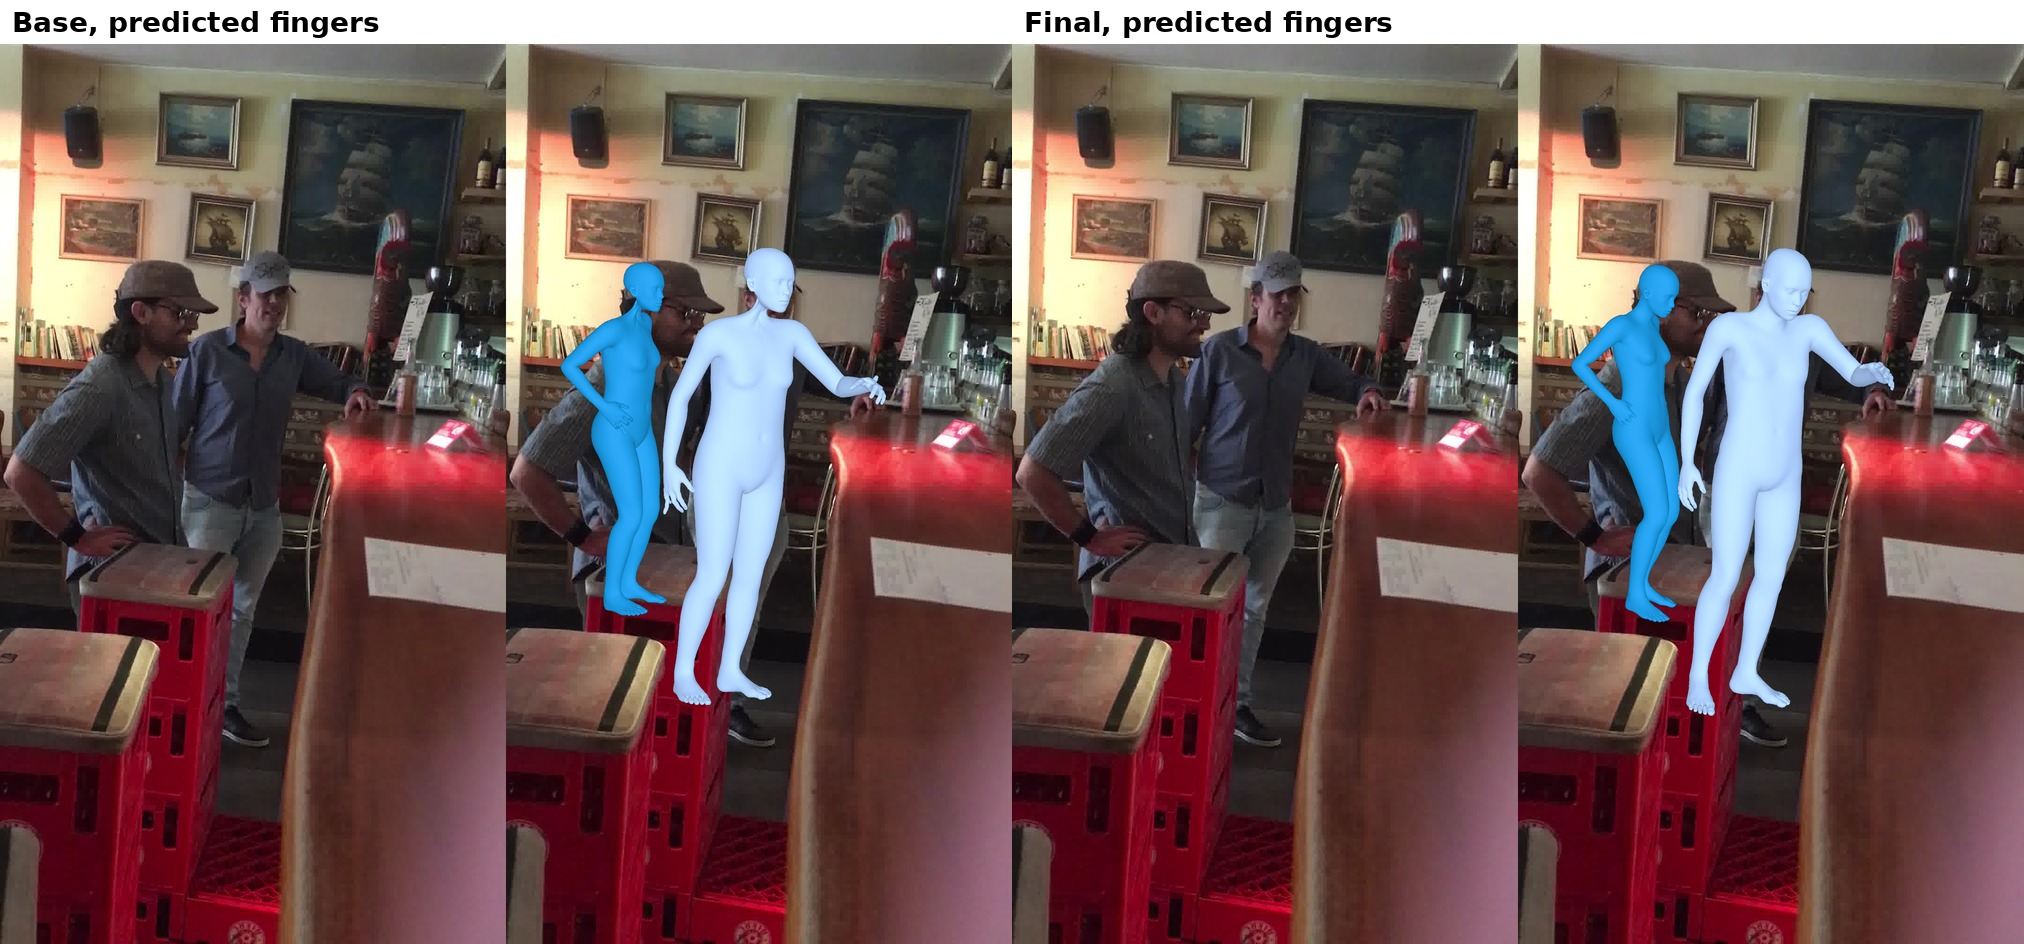
\includegraphics[width=0.288\linewidth]{F11_hands_3dpw_bar}\\[2pt]
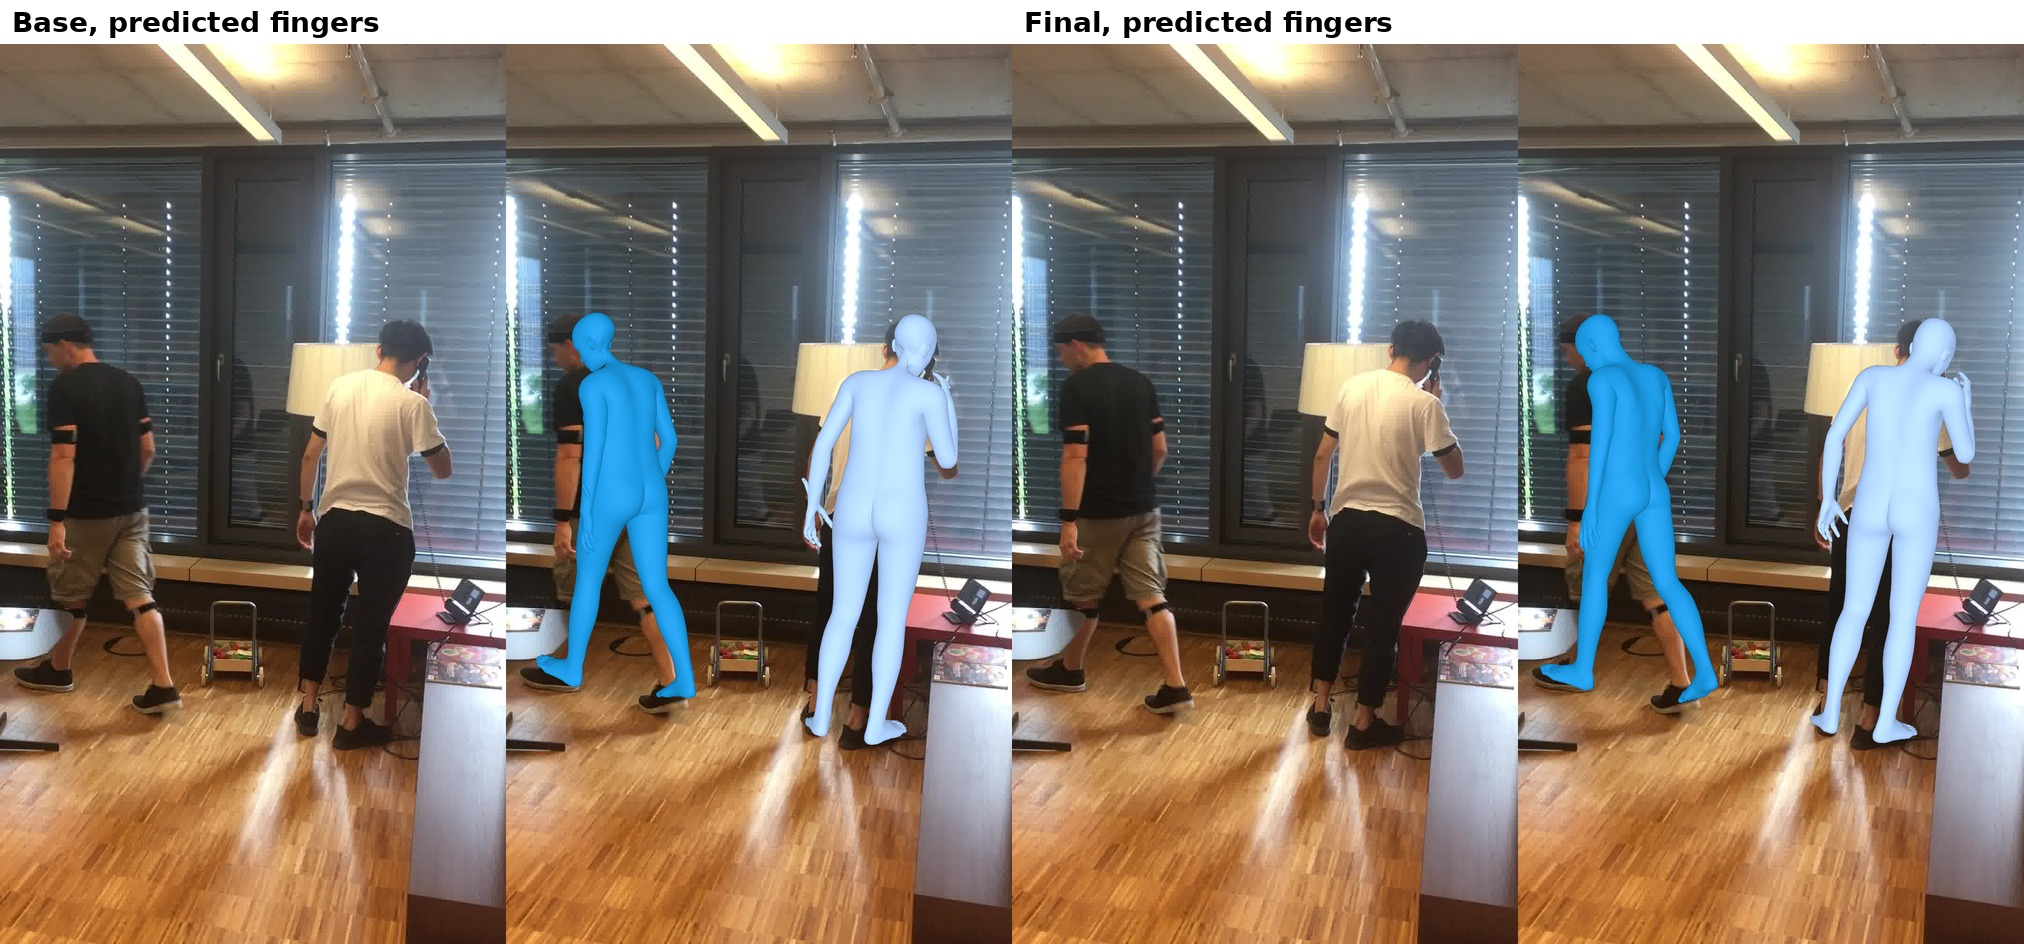
\includegraphics[width=0.288\linewidth]{F11_hands_3dpw_office}\hspace{2pt}%
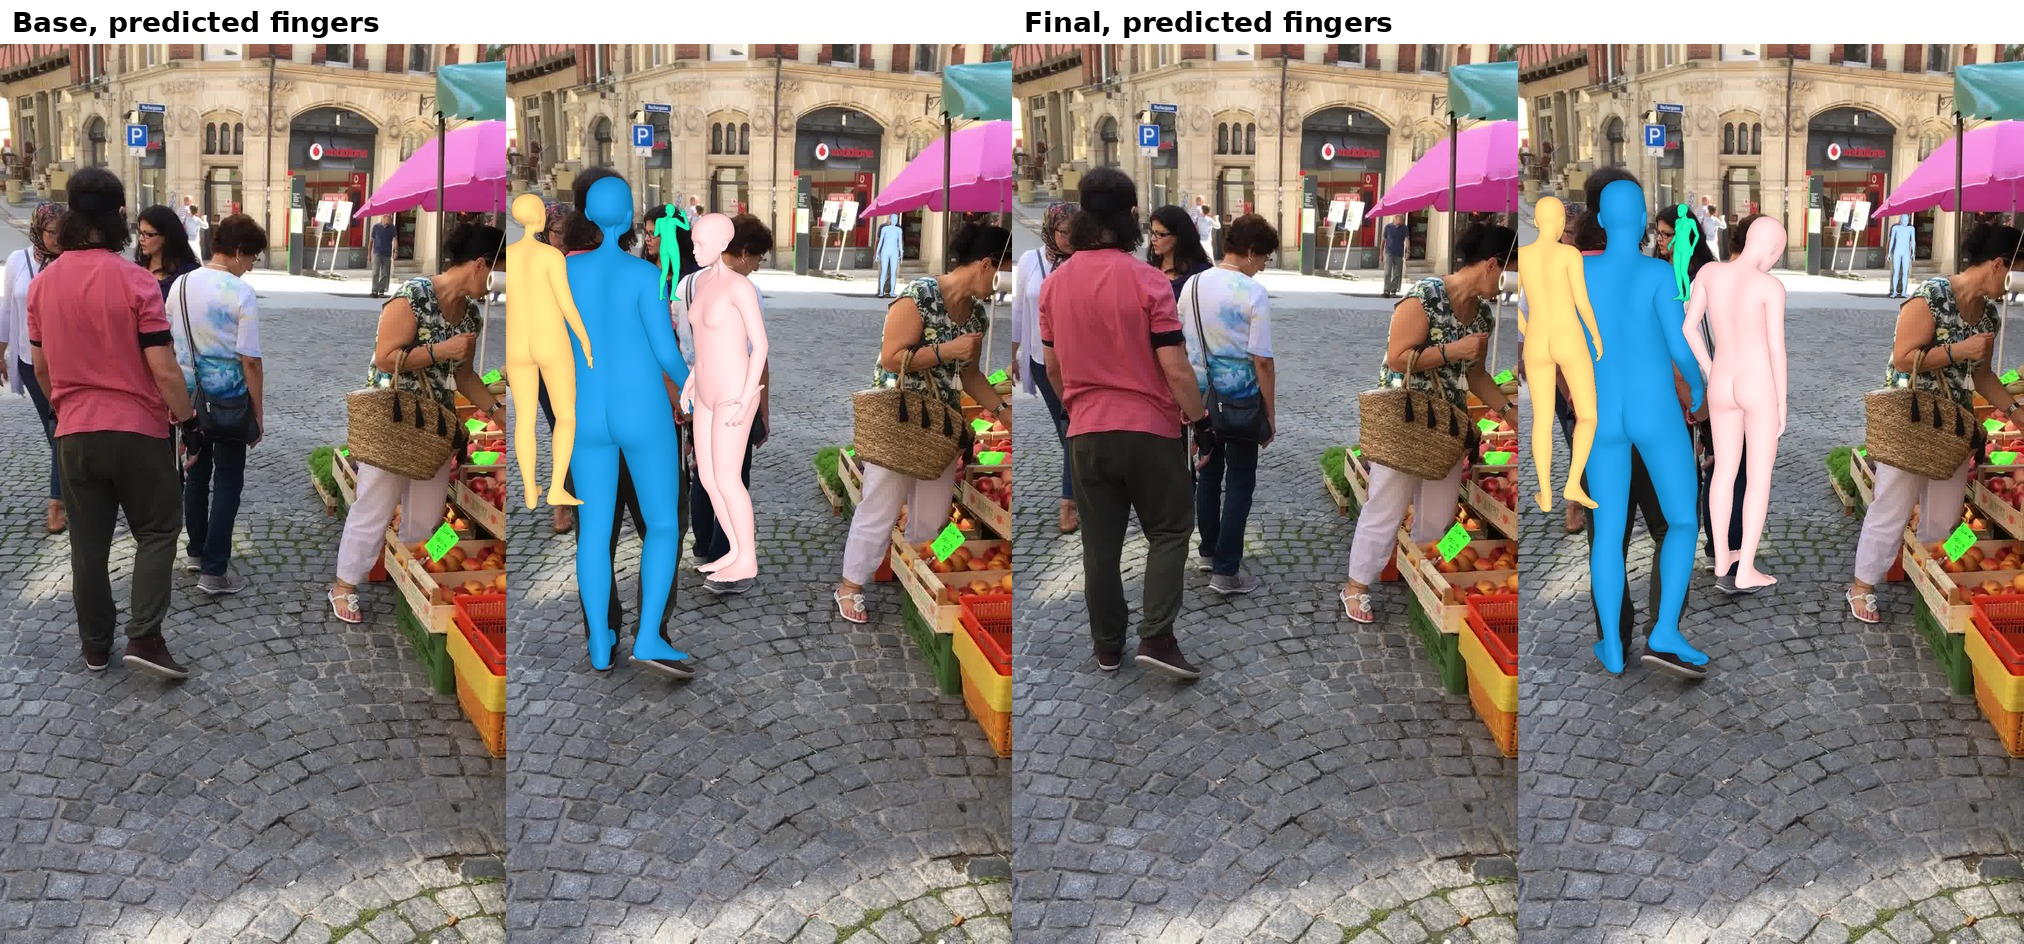
\includegraphics[width=0.288\linewidth]{F11_hands_3dpw_market}
\caption[All twelve demo images with predicted fingers, Base and Final]{All twelve demo images with predicted fingers
(not set to rest pose), each as photo and Base, then photo and Final (labels in the image). Top to bottom: the garden,
tennis and stage photos, the 3DPW test frames fencing, stairs, \texttt{downtown\_walking} and
\texttt{downtown\_runForBus}; then the party photo, guitar, \texttt{downtown\_bar}, \texttt{office\_phoneCall} and
the weekly market. Demo setting, bodies placed from the detector box; Base still has the flipped left index-finger
base (metacarpal1.L) and right ring-finger base, Final has the correction. In most of these images the hands are a
few pixels wide and cannot be judged; Figure~\ref{fig:fingers-demo} zooms on the three where they can. Judged by
eye; no metric.}
\label{fig:fingers-all}
\end{figure}

% F17, the nine rest-pose montages not shown in Chapter 6 (photo | Base | photo | Final | photo | Final-masked,
% labels baked in; demo with --rest_pose 1). Chapter 6 shows tennis, stage and downtown_bar.
\begin{figure}[p]
\centering
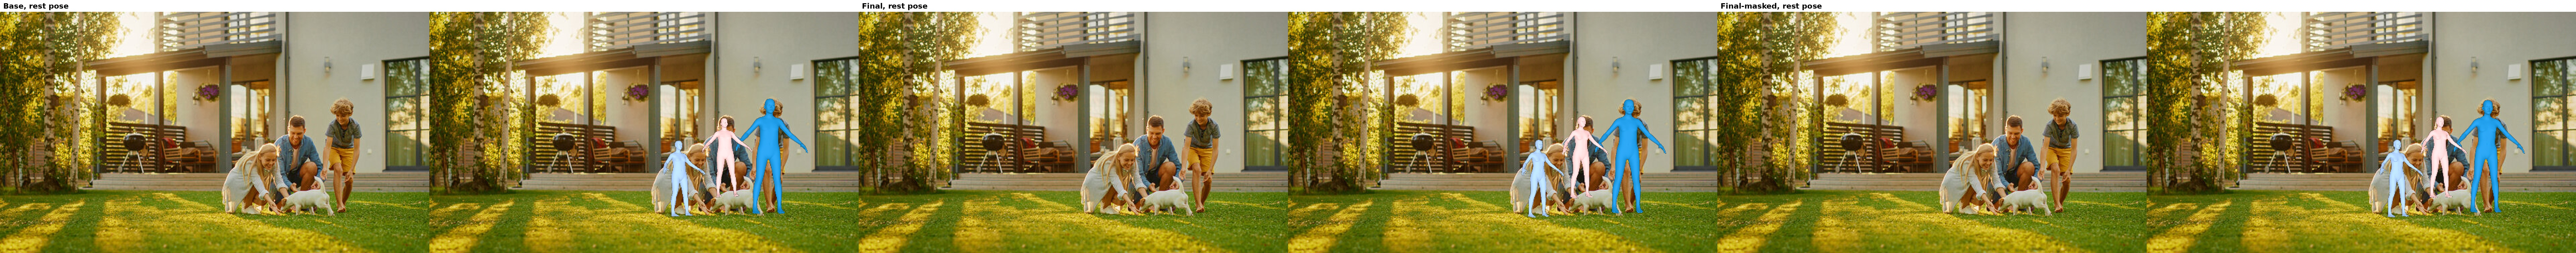
\includegraphics[width=0.9\linewidth]{F17_rest_photo_garden}\\[2pt]
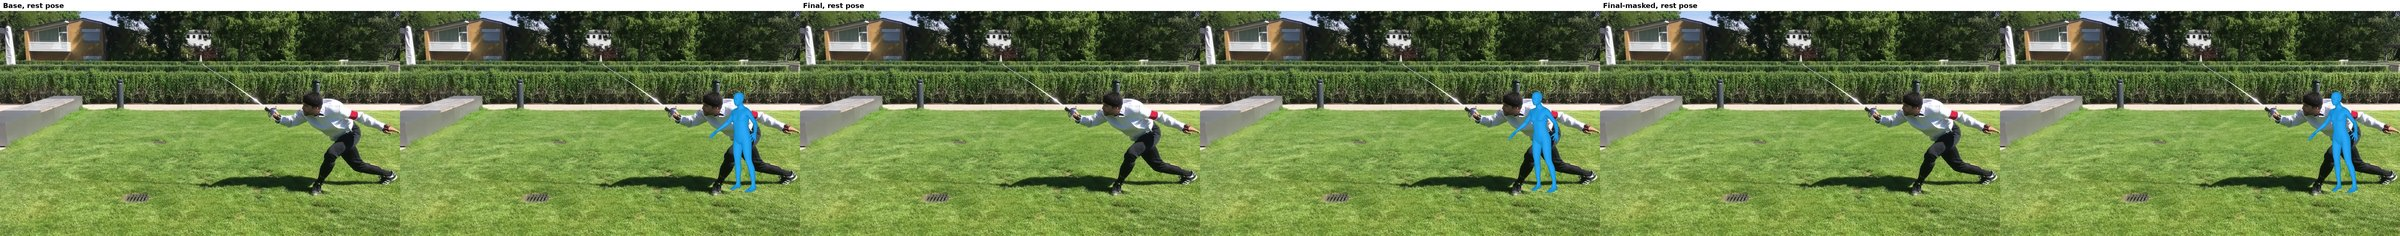
\includegraphics[width=0.9\linewidth]{F17_rest_3dpw_fencing}\\[2pt]
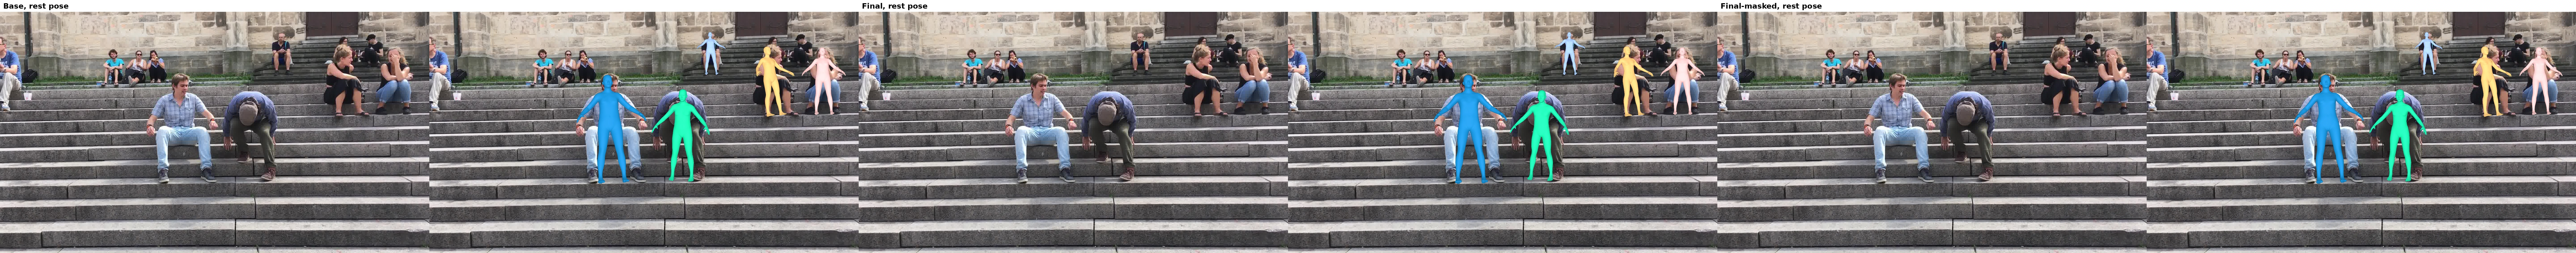
\includegraphics[width=0.9\linewidth]{F17_rest_3dpw_stairs}\\[2pt]
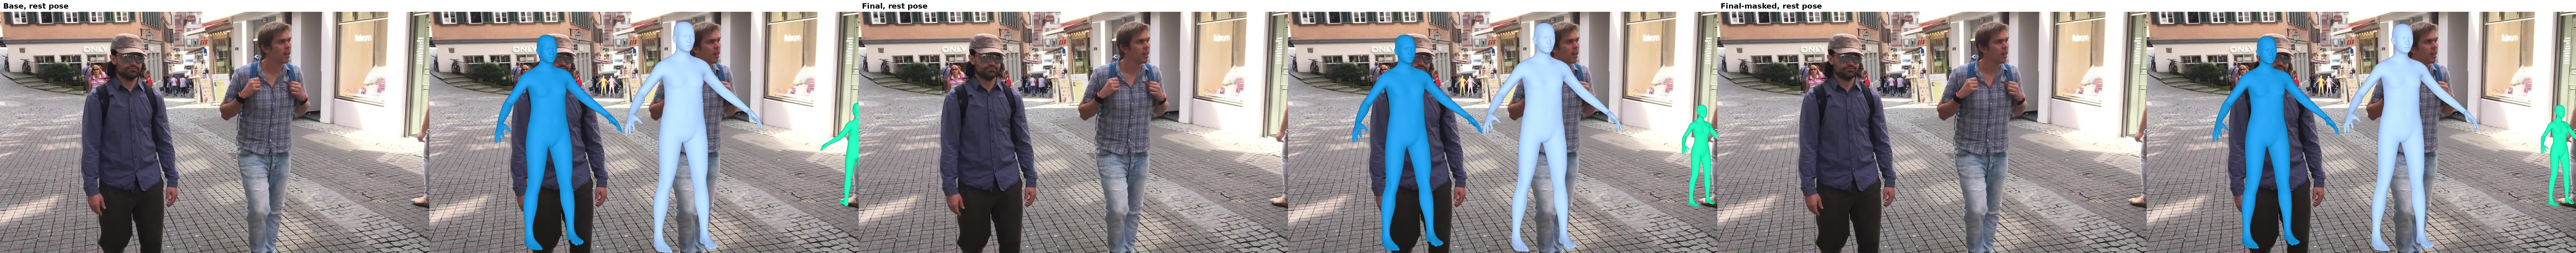
\includegraphics[width=0.9\linewidth]{F17_rest_3dpw_walking}\\[2pt]
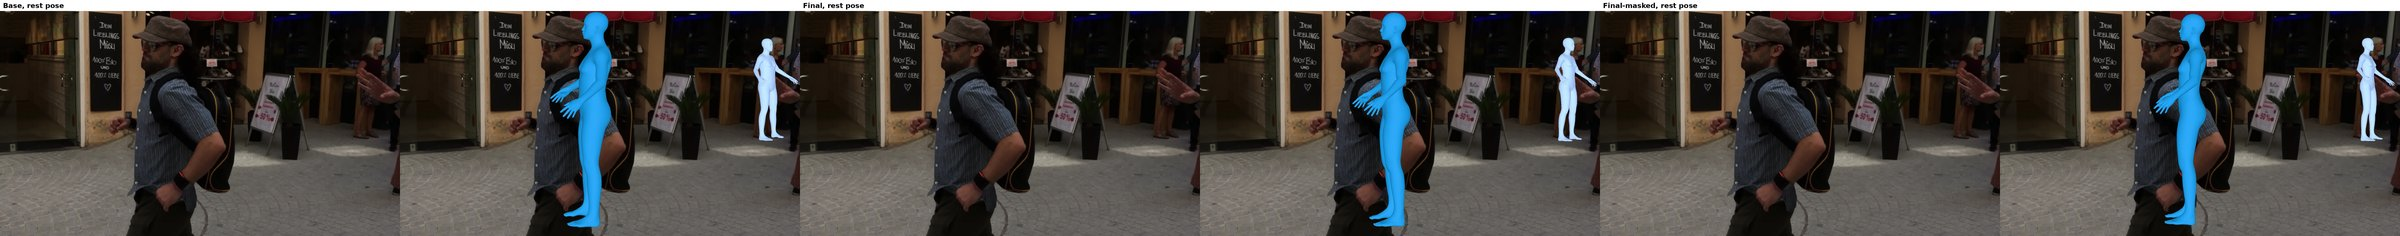
\includegraphics[width=0.9\linewidth]{F17_rest_3dpw_runforbus}\\[4pt]
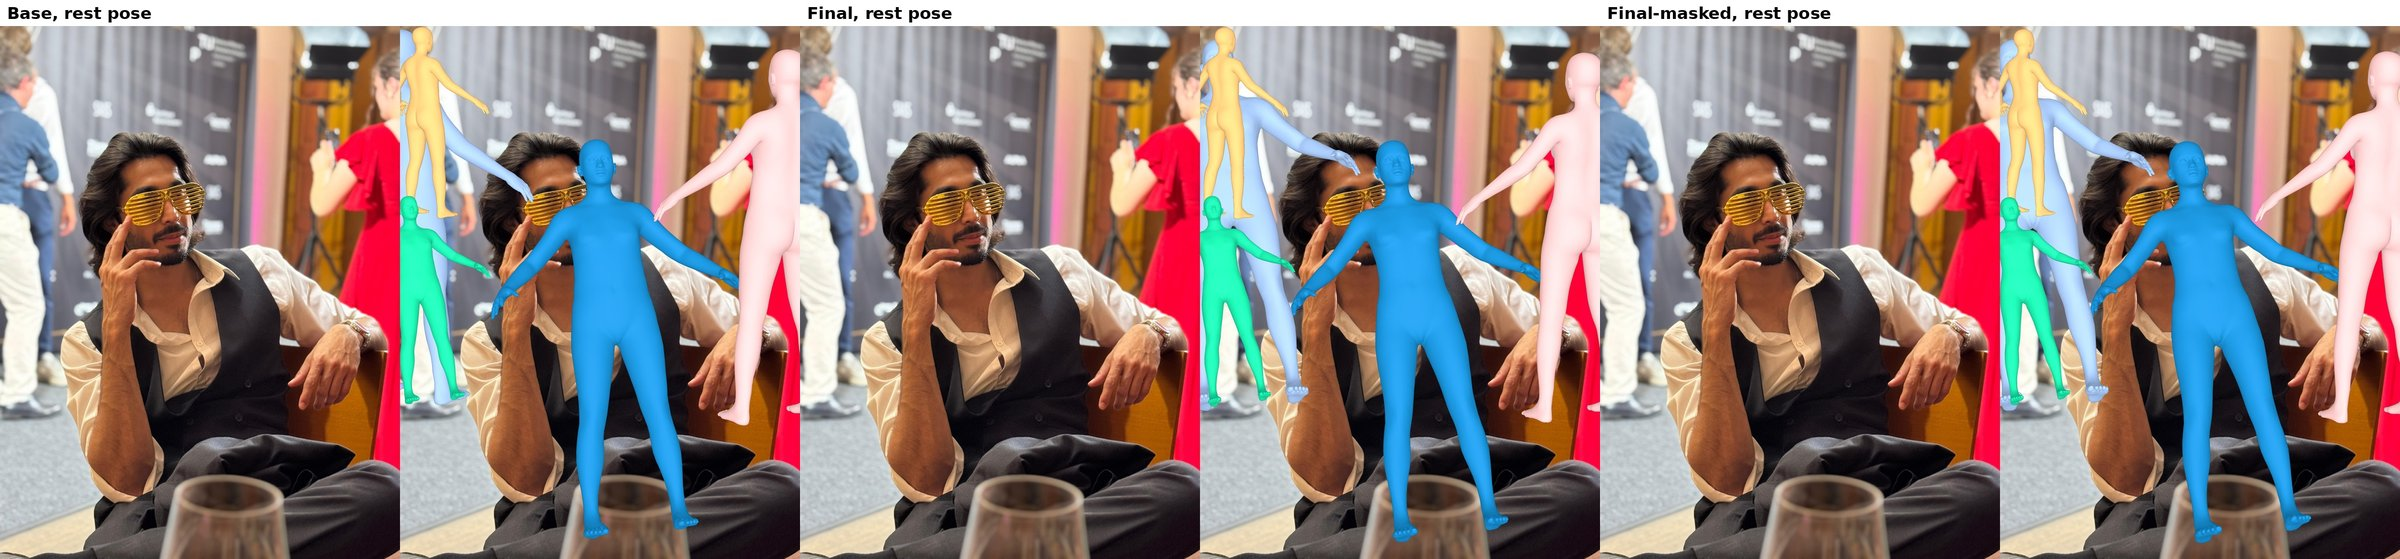
\includegraphics[width=0.495\linewidth]{F17_rest_photo_party}\hfill
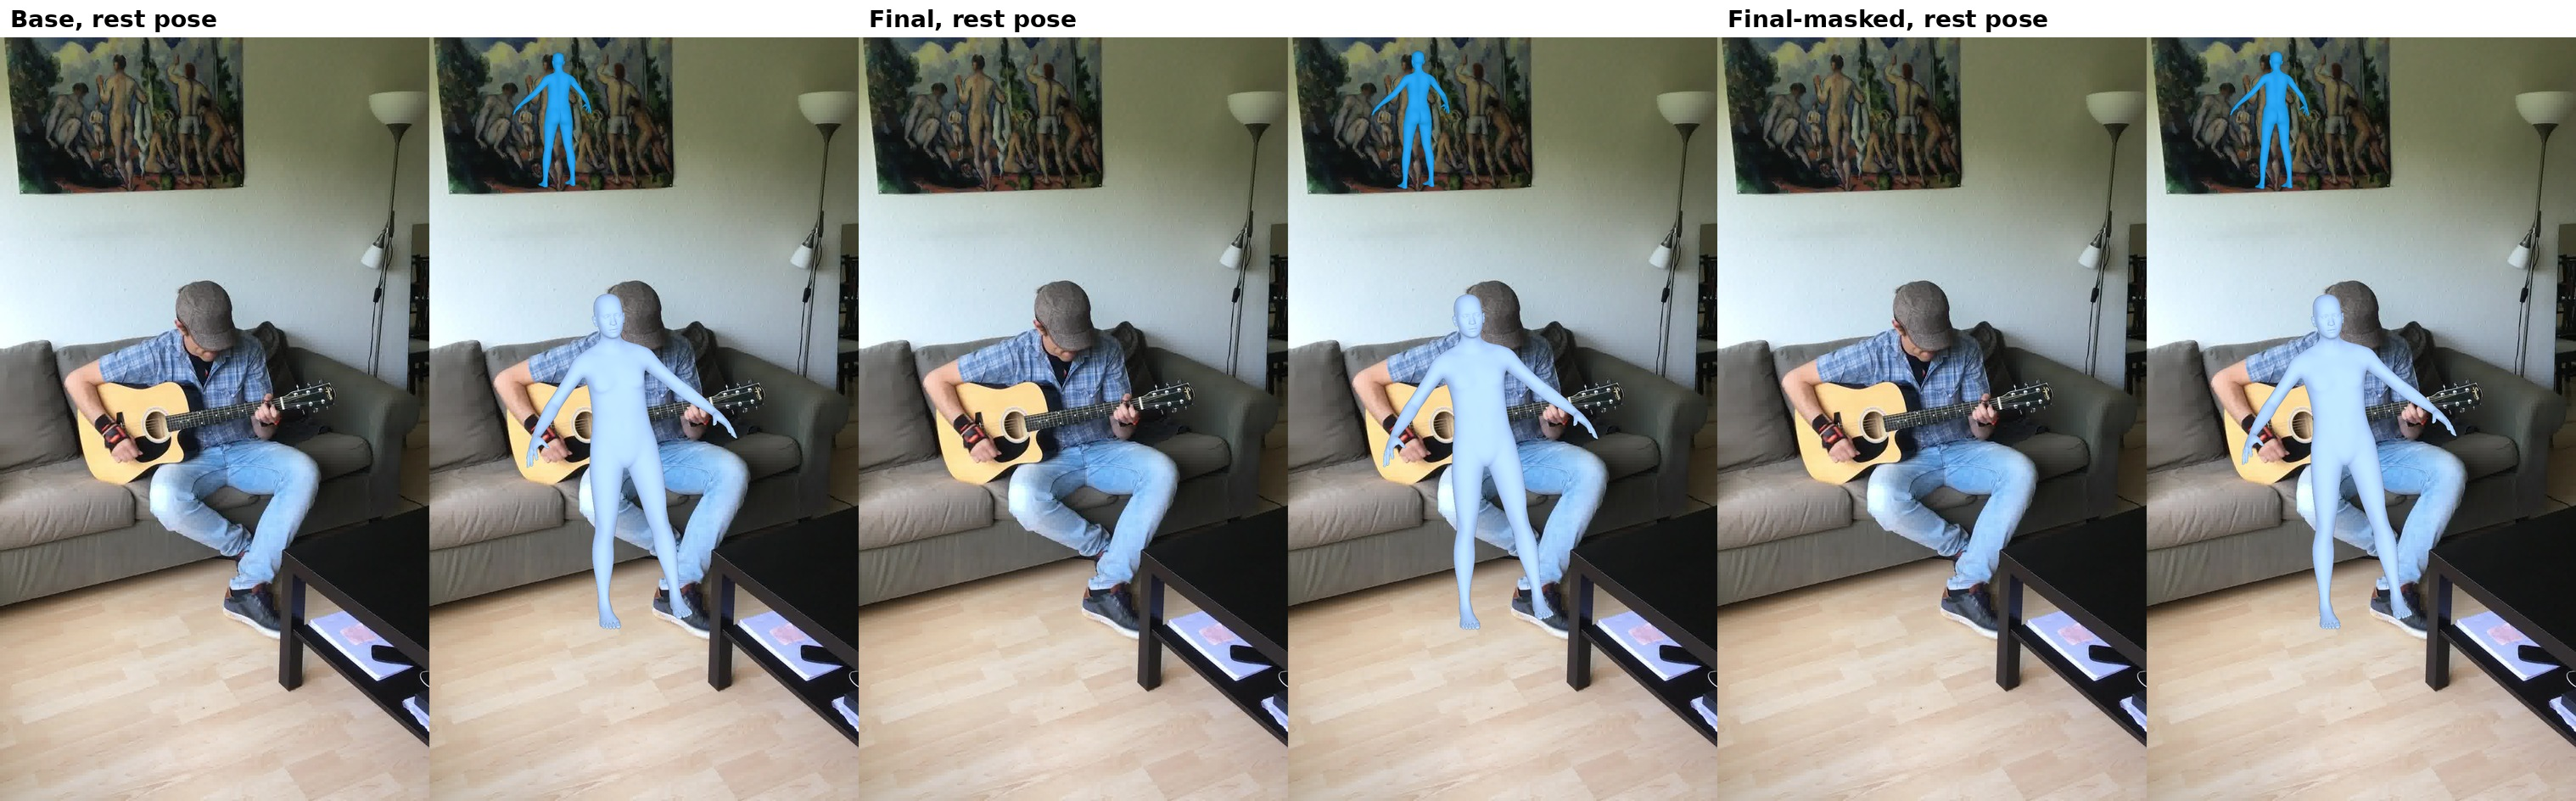
\includegraphics[width=0.495\linewidth]{F17_rest_3dpw_guitar}\\[2pt]
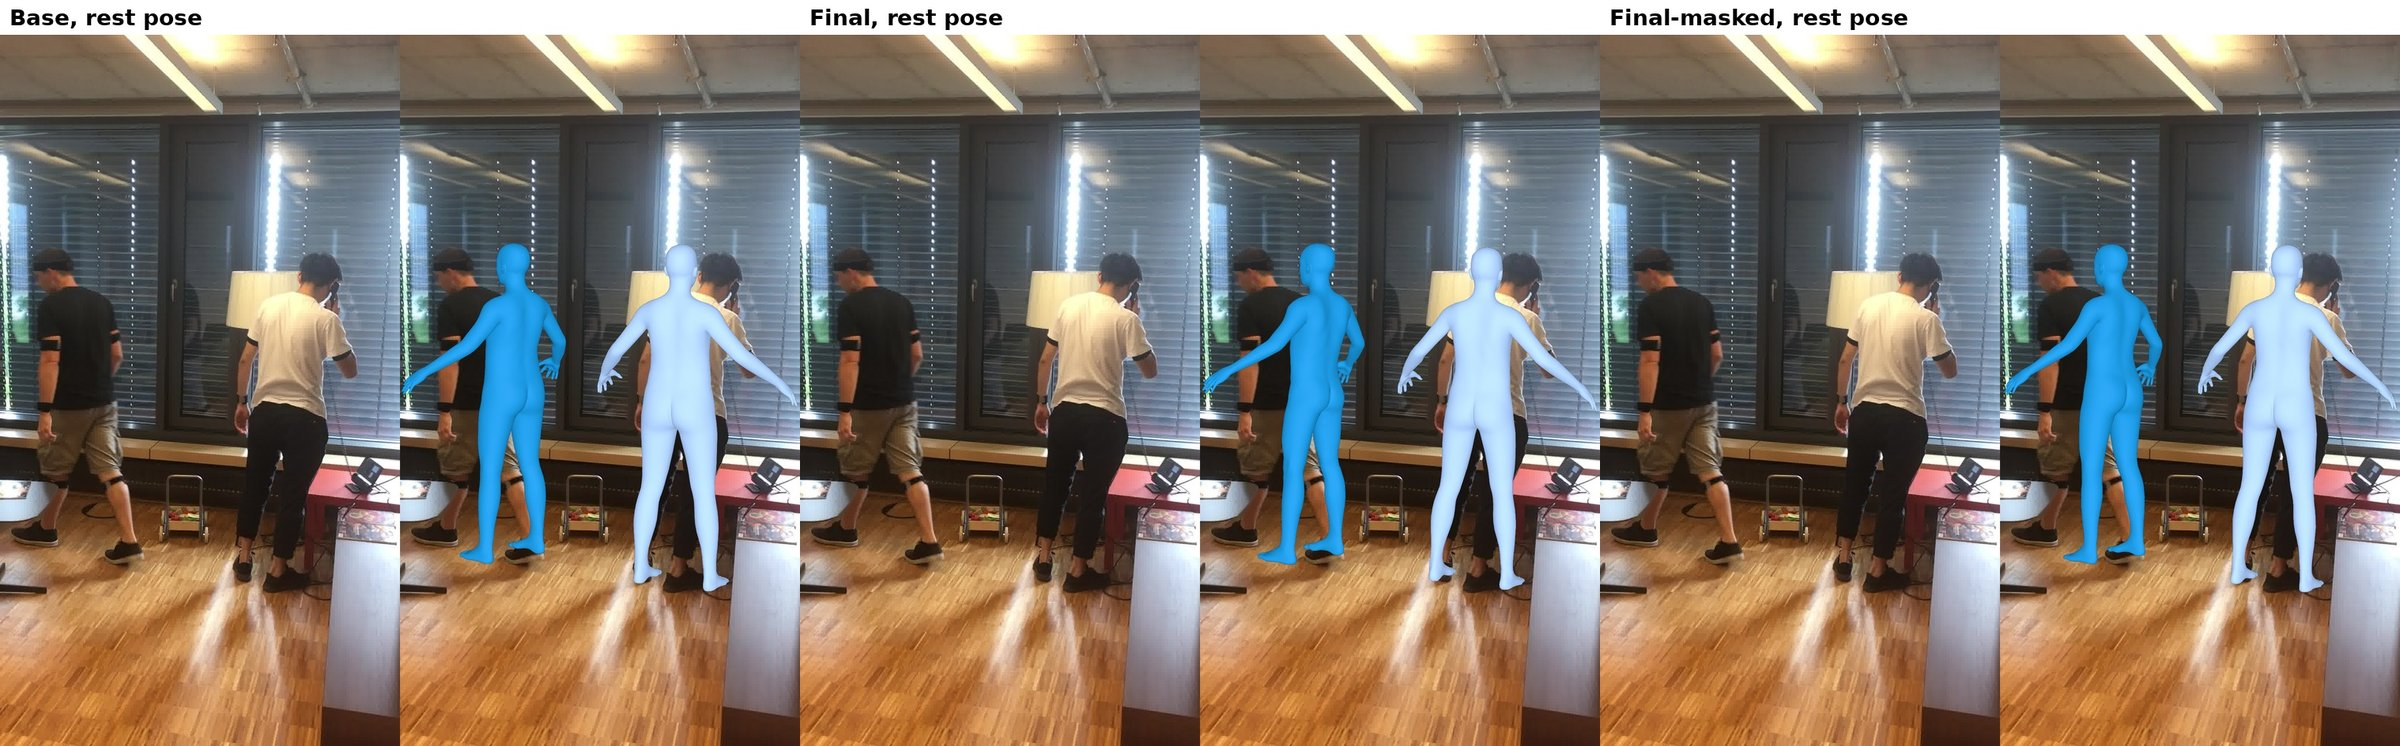
\includegraphics[width=0.495\linewidth]{F17_rest_3dpw_office}\hfill
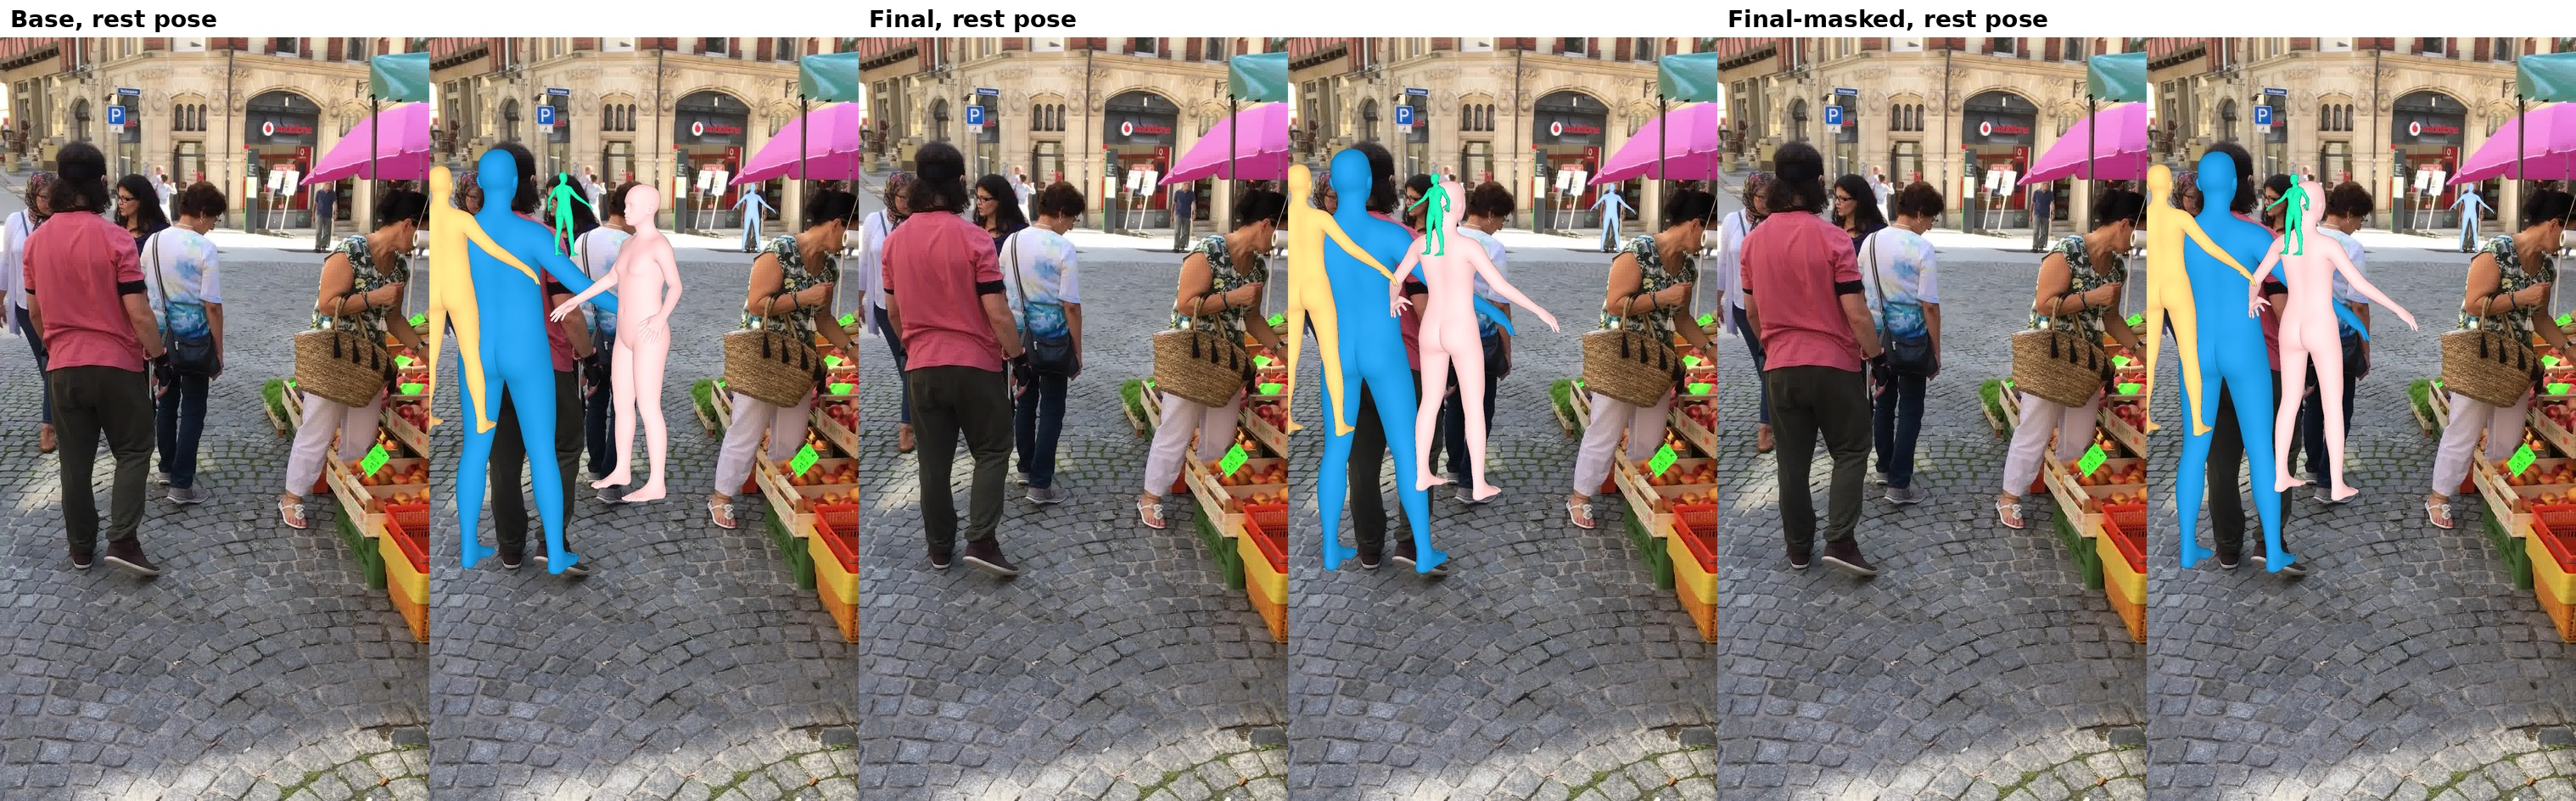
\includegraphics[width=0.495\linewidth]{F17_rest_3dpw_market}
\caption[Nine more rest-pose line-ups: Base, Final, Final-masked]{The other nine demo images in rest pose, each as
photo and Base, photo and Final, photo and Final-masked (labels in the image). Top to bottom: the garden photo, the
3DPW test frames fencing, stairs, \texttt{downtown\_walking} and \texttt{downtown\_runForBus}; then the party photo,
guitar, \texttt{office\_phoneCall} and the weekly market. Every detected person is in rest pose, so only body shape
differs. Demo setting, bodies placed from the detector box; at this size only gross differences of build can be
seen. Judged by eye; no metric. The other three images are in Figure~\ref{fig:rest-lineup}.}
\label{fig:rest-more}
\end{figure}
